\chapter{Upgrades \& the Future of HPS}\label{chap:upgrades}

\begin{figure}
    \centering
    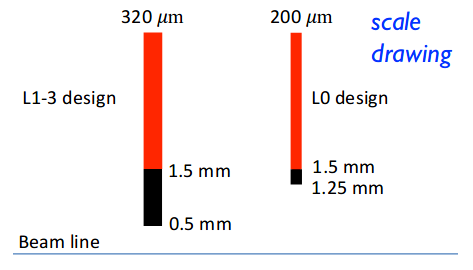
\includegraphics[width=0.45\textwidth]{figs/upgrades/L0_design.png}
    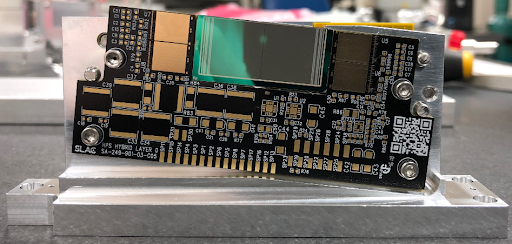
\includegraphics[width=0.45\textwidth]{figs/upgrades/L0.png}
    \caption{Left: A schematic comparing the upgraded L0 sensor dimensions to the nominal sensors used in the other layers. L0 sensors are thinner with far less dead material. Right: A picture of an L0 thin sensor full module (stereo side) and hybrid circuit.}
    \label{fig:L0}
\end{figure}

\begin{figure}
    \centering
    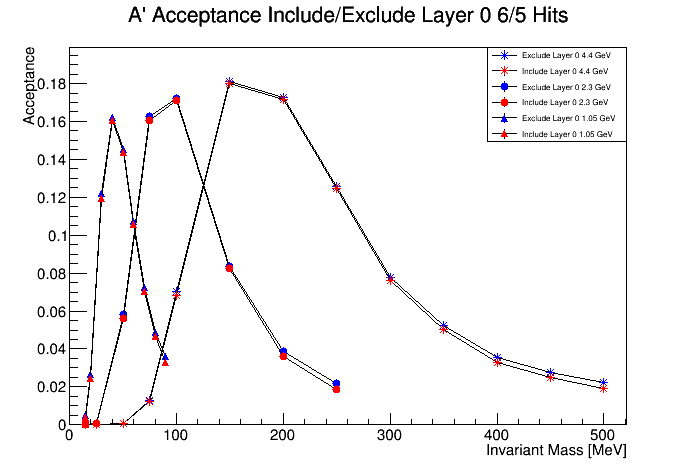
\includegraphics[width=0.45\textwidth]{figs/upgrades/TridentAcceptanceInL0ExL05hit.png}
    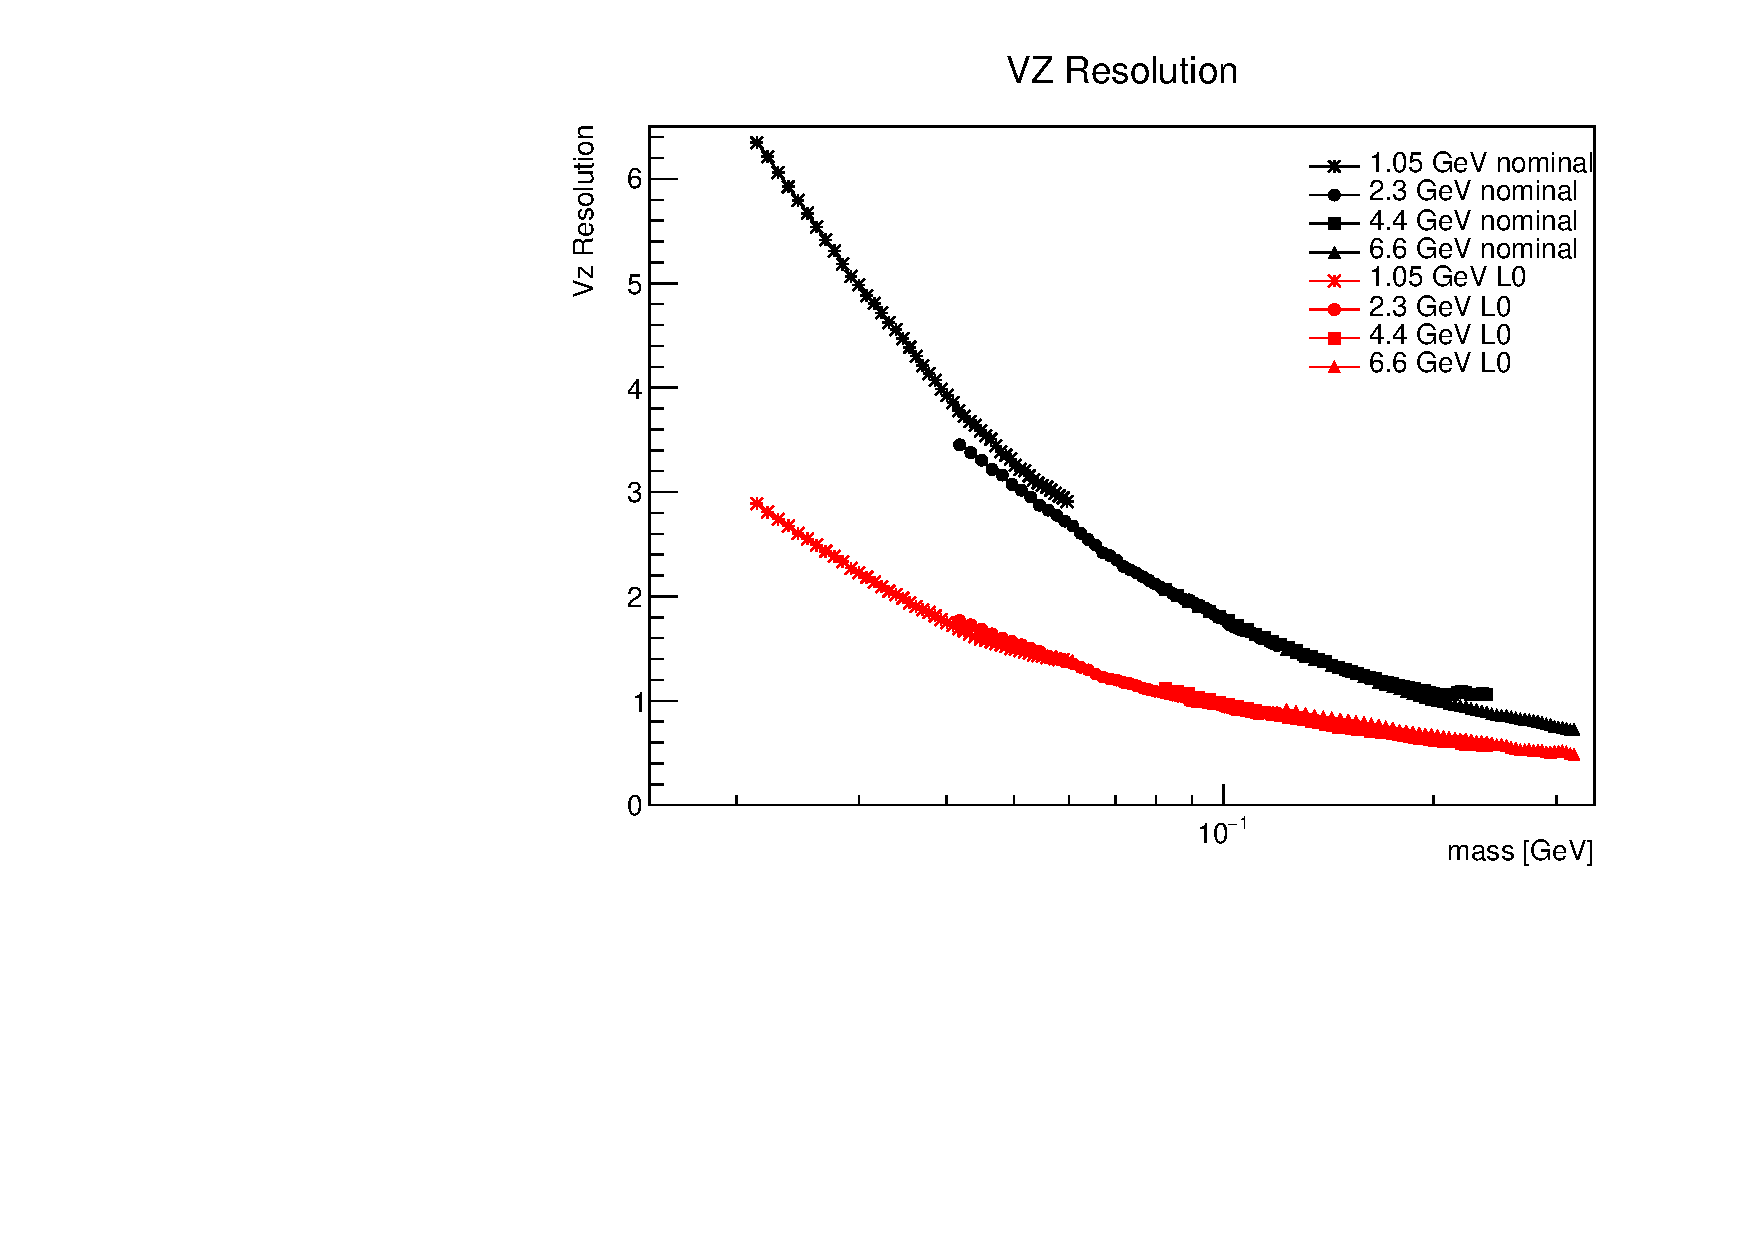
\includegraphics[width=0.45\textwidth]{figs/upgrades/VZ_Resolution_total.pdf}
    \caption{Left: A comparison of the acceptance for prompt trident events for the nominal detector and the upgraded L0 detector. The acceptance is remarkably close despite the smaller L0 sensor dimensions (the acceptance is concentrated on the center of the sensor near the beam edge). Right: A comparison of the vertex resolution with the nominal detector and upgraded L0 detector. The improvement in vertex resolution is about a factor of 2.}
    \label{fig:L0acceptance}
\end{figure}

%\begin{figure}
%    \centering
%    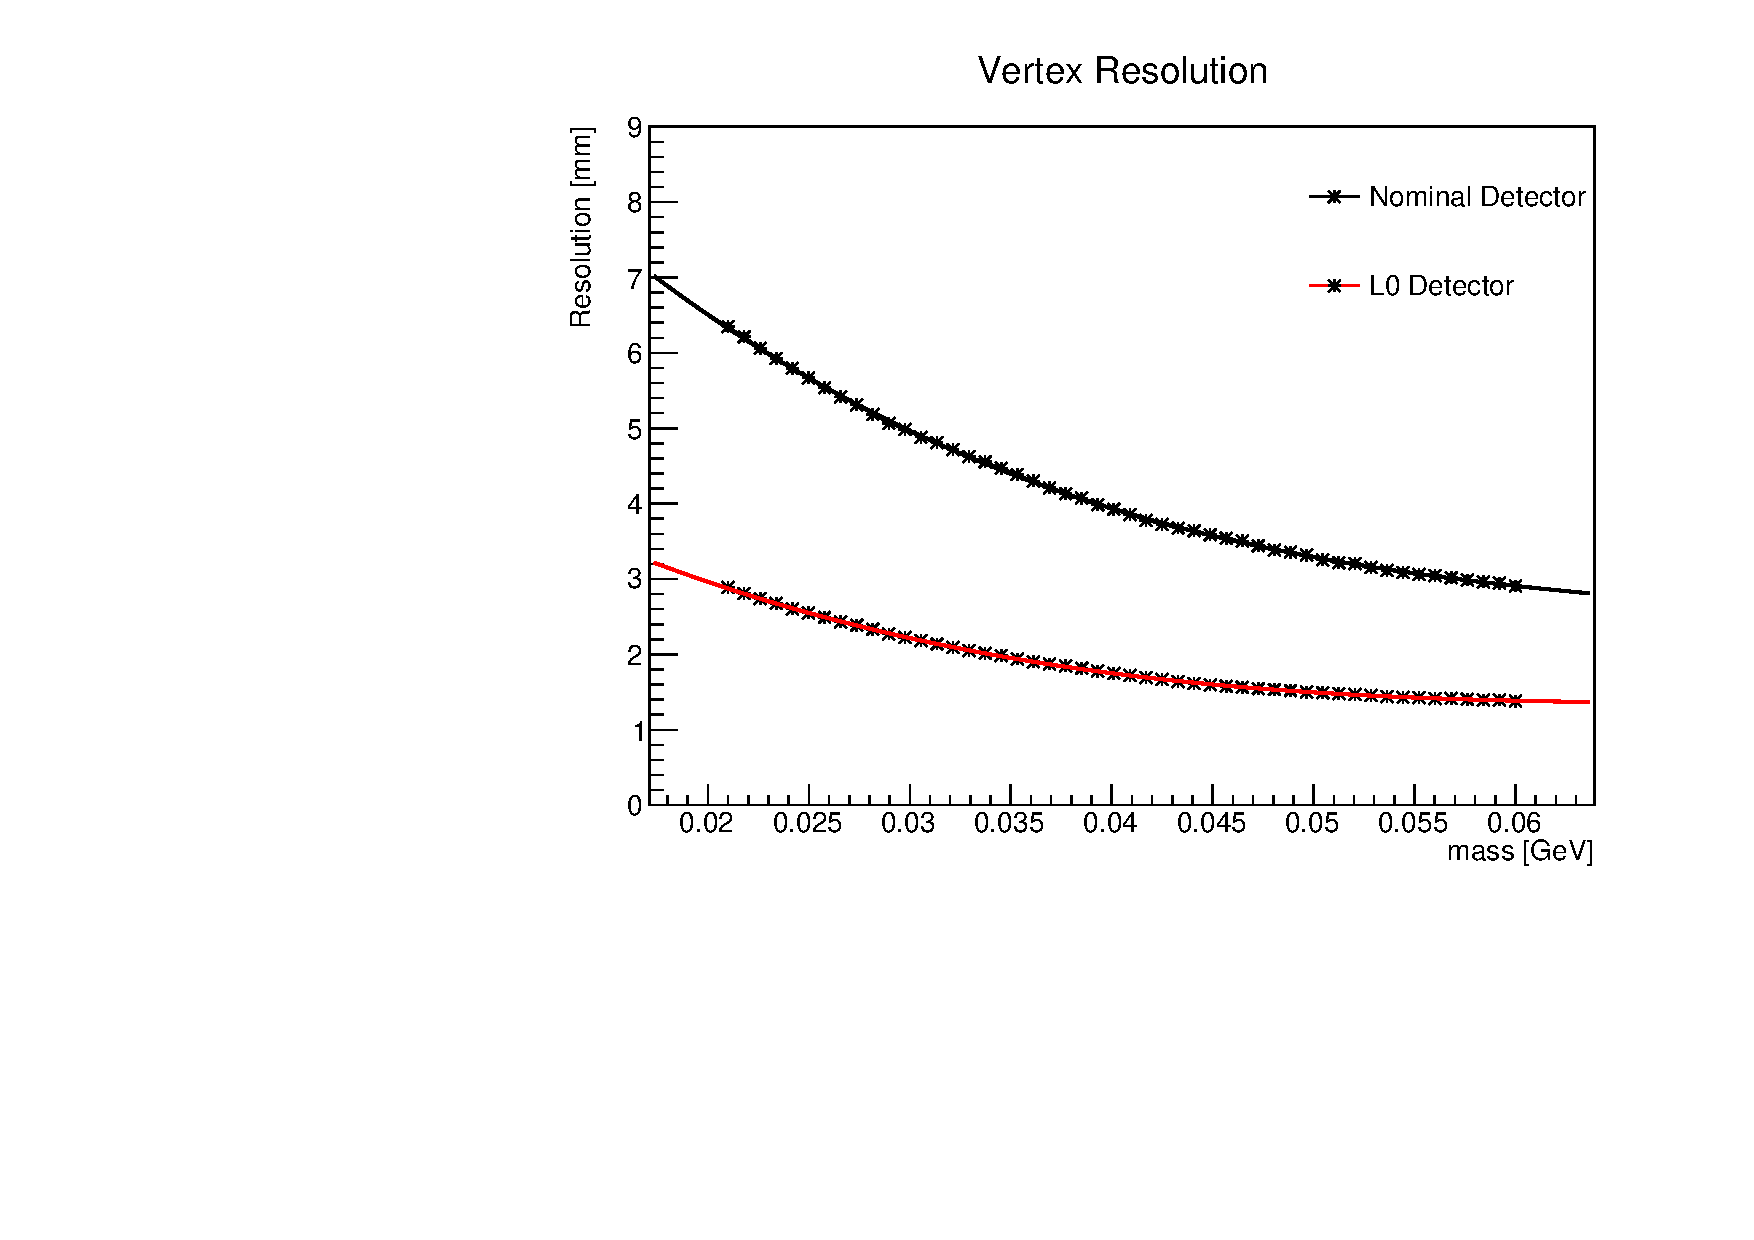
\includegraphics[width=0.5\textwidth]{figs/upgrades/VZ_Resolution_1pt05.pdf}
%    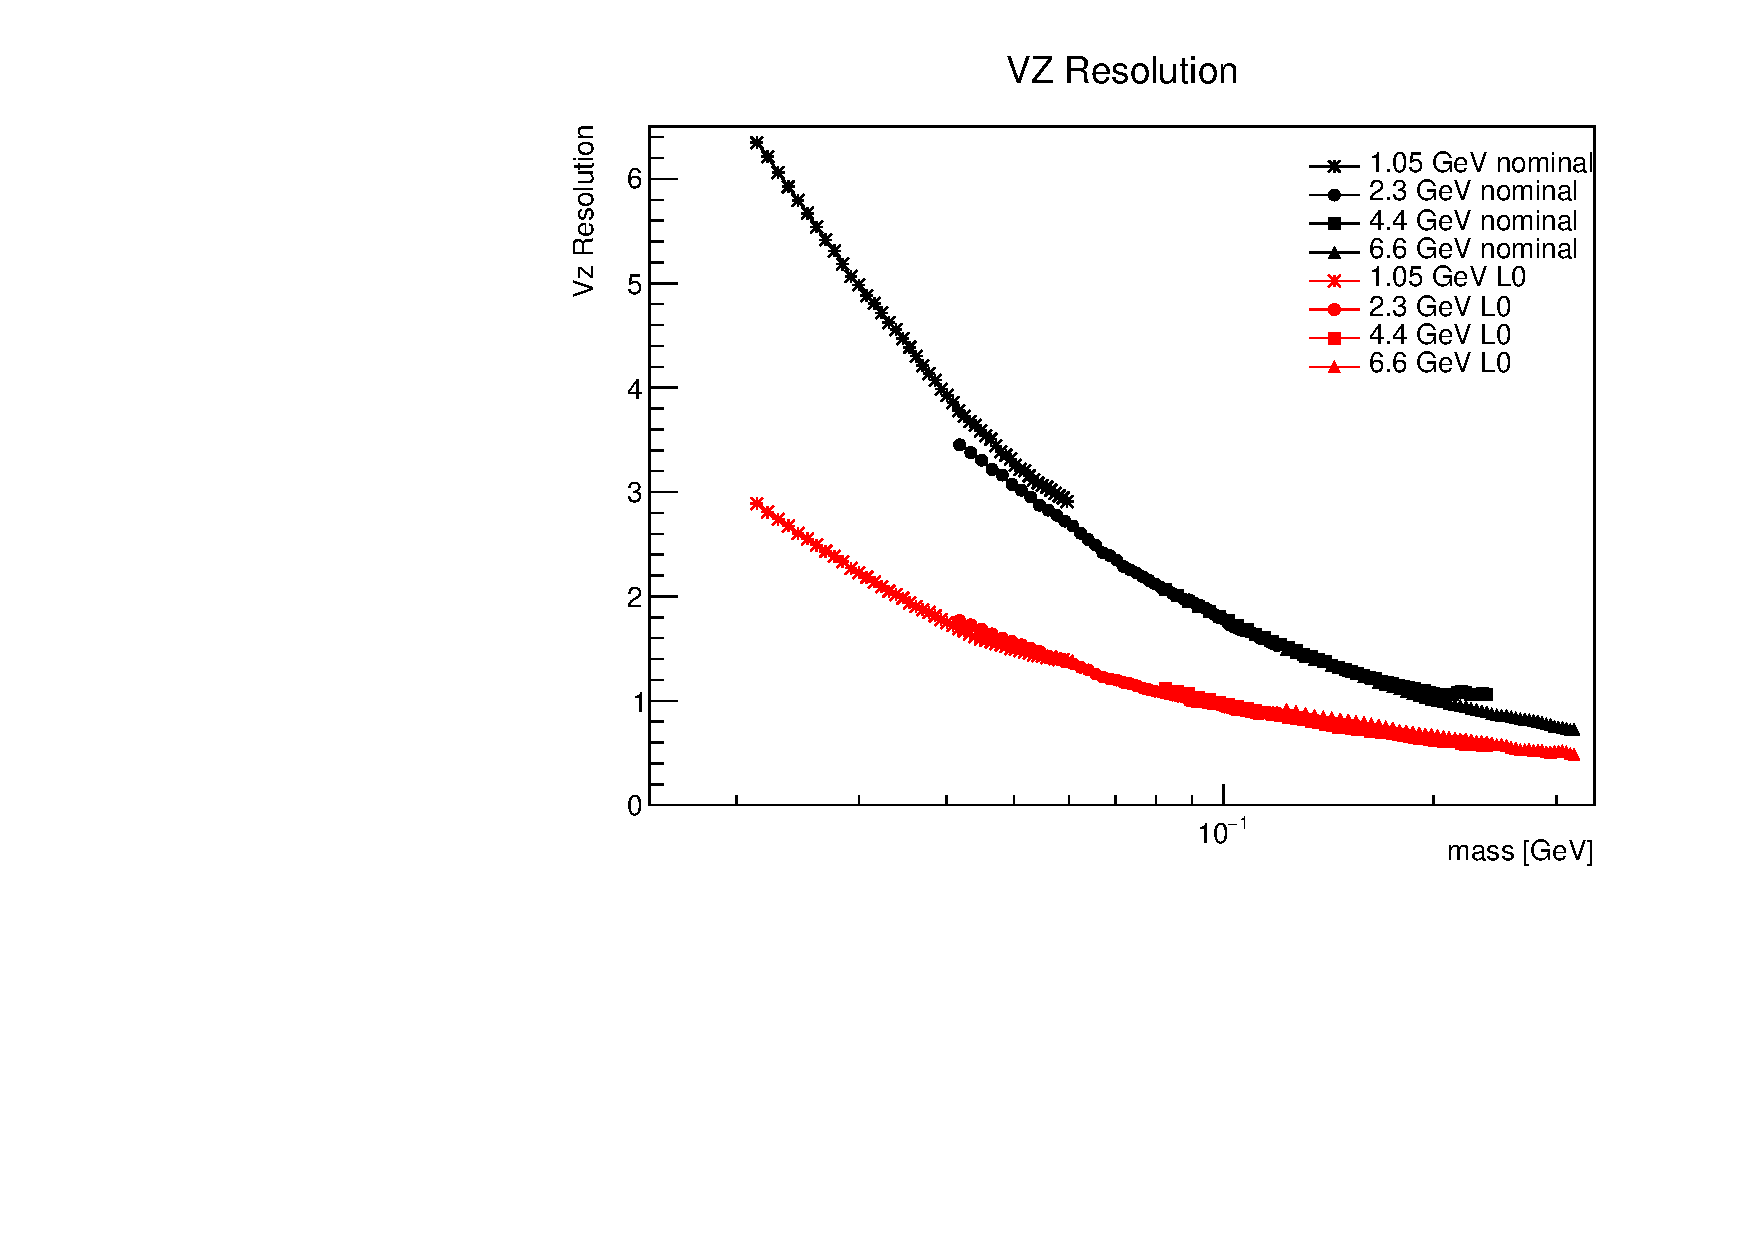
\includegraphics[width=0.5\textwidth]{figs/upgrades/VZ_Resolution_total.pdf}
%    \caption{VZ Resolution.}
%    \label{fig:L0resolution}
%\end{figure}

Beyond what was shown in this thesis, which focused on the results of the 2016 Engineering Run, the future of HPS is promising and includes much more running time with an upgraded detector. The two engineering runs only account for about $\sim$4\% of the total allotted running time of 180 days. In addition, HPS has recently completed its first physics run during the summer of 2019. For this run, the displaced vertex search result in both the 2015 and 2016 Engineering Runs motivated the need for several upgrades. With the current detector configuration, it would take at least 8 weeks with the displaced vertex search to achieve any sensitivity to the canonical $\aprime$ model. However, several simple upgrades that improve vertex resolution and increase $\aprime$ acceptance make long-lived $\aprime$ searches possible on a much shorter time scale.

In addition to upgrades, HPS is able to probe a unique region of parameter space involving short livetimes and small cross-sections. Essentially, HPS is able to measure livetimes, cross-sections, and masses of long-lived particles and it can potentially probe any model containing electro-produced long-lived particles that decay into $\epem$ pairs. There are other models that fit this requirement and in the future HPS will move to a generalized displaced vertex search to test all these models. One such model is presented in this chapter.

\section{Upgrade Simulations and Installation}\label{sec:L0}

In order to achieve the full effectiveness of HPS, several simple upgrades were implemented for the most recent 2019 Physics Run. Informed by analysis from the previous two engineering runs, three simple upgrades were added - the addition of a tracking layer between the current layer 1 and the target, the implementation of a hodoscope which enabled a positron trigger, and the movement of the current L1-L3 more towards the beam plane.

The additional tracking layer, approximately halfway between the current layer 1 and the target (hence the name ``layer 0'' or ``L0''), improves the vertex resolution. Since the vertex resolution is dominated by multiple scattering in the first layer and the additional tracking layer cuts the distance between the target and the first measurement plane in half, the vertex resolution improves by about a factor of two. The improvement of vertex resolution allows for a significantly larger signal region (a $z_{cut}$ closer to the target), and since the signal shape is exponential in $z$, this dramatically improves the physics potential for the displaced vertex search. A comparison between the nominal detector and the upgraded L0 detector for acceptance as well as a comparison of the vertex resolution is shown in Fig. \ref{fig:L0acceptance}.

There are several technical challenges associated with adding another tracking layer closer to the target. In order to maintain the same geometrical acceptance for prompt processes at 15 mrad, the active edge of the axial L0 sensor must be placed at half the distance from the current location of L1 (from 1.5 mm to 0.75 mm). However, this would place the guard ring (i.e. the inactive silicon) of the existing sensors directly into the beam plane which is obviously not feasible due to radiation. To accommodate this, new sensors were designed with a slim edge in which the dead region is only 0.25 mm instead of 1.0 mm. This places the physical edge of the silicon at the original layer 1 vertical position of 0.5 mm from the beam plane while the active edge is placed at 0.75 mm from the beam plane to maintain 15 mrad prompt acceptance.

The closer placement of the L0 active sensor to the beam plane presents challenges for occupancy. For this reason, the sensors are split in two left-right halves such that each half contains strips and the sensors are readout at both ends. This effectively cuts the occupancy in half to a similar level of the layer 1 sensors in the nominal tracker. Lastly, the L0 sensor is thinner at 200 $\mu$m compared to the nominal of 320 $\mu$m which further reduces multiple scattering effects. A schematic and picture of the L0 sensors are shown in Fig. \ref{fig:L0}.

In addition to the new tracking layer, layers 2 and 3 in the tracker were moved closer to the beam plane in order to increase acceptance of $\aprime$s that live long enough and miss the first layer in the tracker (L0 in this case). Specifically layers 2 and 3 were moved 700 $\mu$m closer to beam by placing a simple mechanical shim in the U-channels underneath the layer 2 and 3 modules. The effect for increasing acceptance for $\aprime$s that decay past about $\sim 70$ mm is shown in Fig. \ref{fig:40MeVeff}.

After the initial studies described below were performed, in addition to moving layers 2 and 3 closer to the beam, it was decided that it would be beneficial for the current layer 1 modules to be replaced with the thin sensor modules designed for layer 0. This has several advantages. First, the thinner silicon material reduces multiple scattering. Second, the slim edge in these sensors allows for a closer placement of the sensor to the beam plane thus increasing the acceptance to $\aprime$s that decay beyond the L0 acceptance.\footnote{After the nominal module was replaced by a thin sensor, layer 1 was moved 400 $\mu$m closer to the beam which means the silicon edge is still 850 $\mu$m from the beam plane.} As a minor disadvantage, there is some acceptance loss to recoil electrons (which are generally soft), though there is minimal acceptance losses for $\aprime$ daughters. %These initial MC studies do not have these changes to the layer 1 configuration.

\begin{figure}
    \centering
    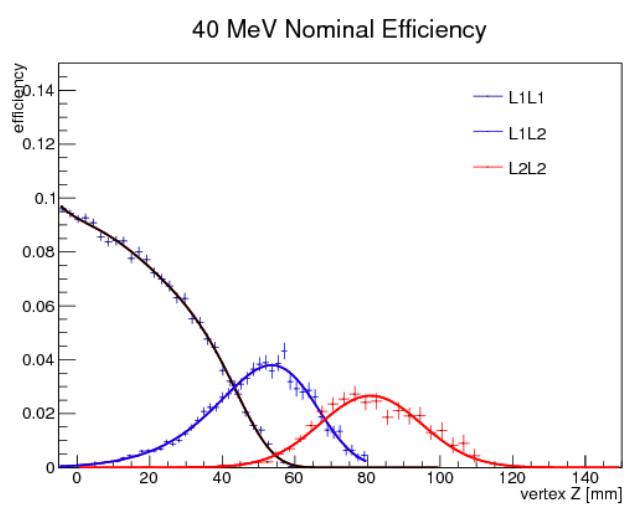
\includegraphics[width=0.45\textwidth]{figs/upgrades/40MeV_nominal_eff.png}
    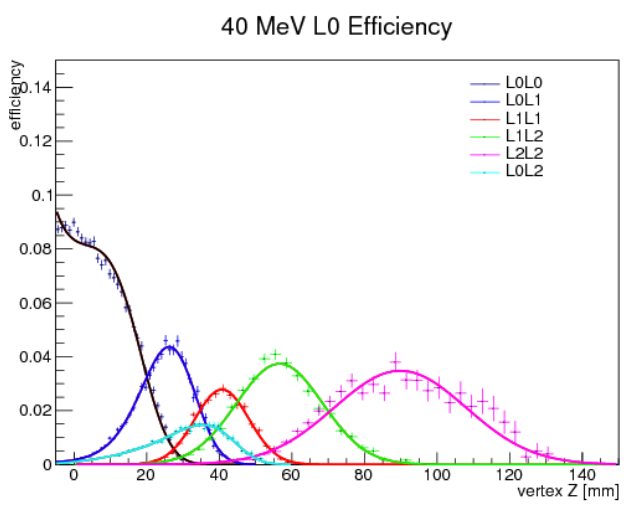
\includegraphics[width=0.45\textwidth]{figs/upgrades/40MeV_L0_eff.png}
    \caption{The efficiency of a displaced 40 MeV $\aprime$ separated into different mutually exclusive categories based on the first layer hit by the positrons and electrons for both the nominal and L0 upgraded detector. Left: The nominal detector separated in to L1L1, L1L2, and L2L2. Right: The upgraded L0 detector separated into L0L0, L0L1, L1L1, L0L2, L1L2, and L2L2.}
    \label{fig:L0eff}
\end{figure}

\begin{figure}
    \centering
    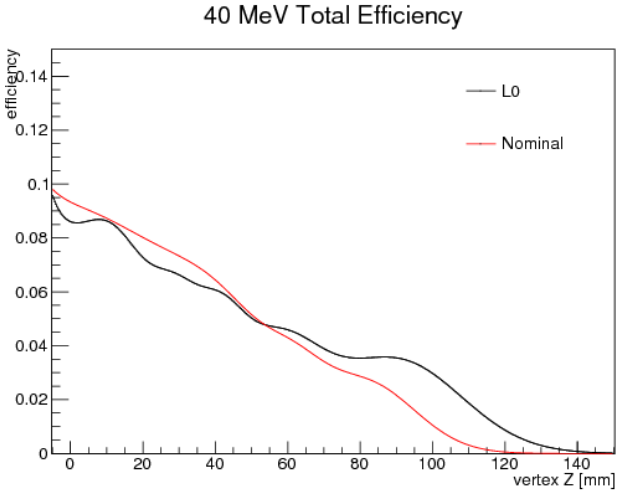
\includegraphics[width=0.5\textwidth]{figs/upgrades/40MeV_tot_eff.png}
    \caption{A comparison for a 40 MeV displaced $\aprime$ of the total efficiency (including acceptance effects) between the nominal detector and the upgraded detector by adding the mutually exclusive categories in Fig. \ref{fig:L0eff}. The L0 has increased acceptance for large $z$ due to layers 2 and 3 in the tracker being moved closer to the beam. There may be some additional acceptance losses for $z<50$ mm for the L0 detector due to multiple scattering in the inactive silicon.}
    \label{fig:40MeVeff}
\end{figure}

Lastly, a hodoscope was added between the tracker and the Ecal. As described in Sec. \ref{sec:ecal}, the nominal trigger was tuned to $\epem$ pairs of $\aprime$ daughter particles. However, the Ecal was constructed in such a way that five crystals at the beam edge in each of the top and bottom halves were removed to decrease occupancy from beam particles. This is called the ``Ecal hole'' or ``Ecal gap'' and is shown in Fig. \ref{fig:ecal}. Unfortunately, about half of the prompt $\aprime$ acceptance is contained in these few crystals and more so for low mass $\aprime$s. And because there is still acceptance with the tracker in this region, a positron-only trigger will recover the events where electrons are lost in the Ecal gap. Adding a hodoscope on the positron side allows for matching hits in the hodoscope with crystals in the Ecal; this suppresses triggers from single photons on the positron side, increases acceptance, and leads to manageable trigger levels. This is shown in Fig. \ref{fig:positrigger}.

\begin{figure}
    \centering
    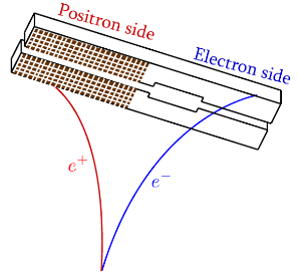
\includegraphics[width=0.45\textwidth]{figs/upgrades/positron_trigger.png}
    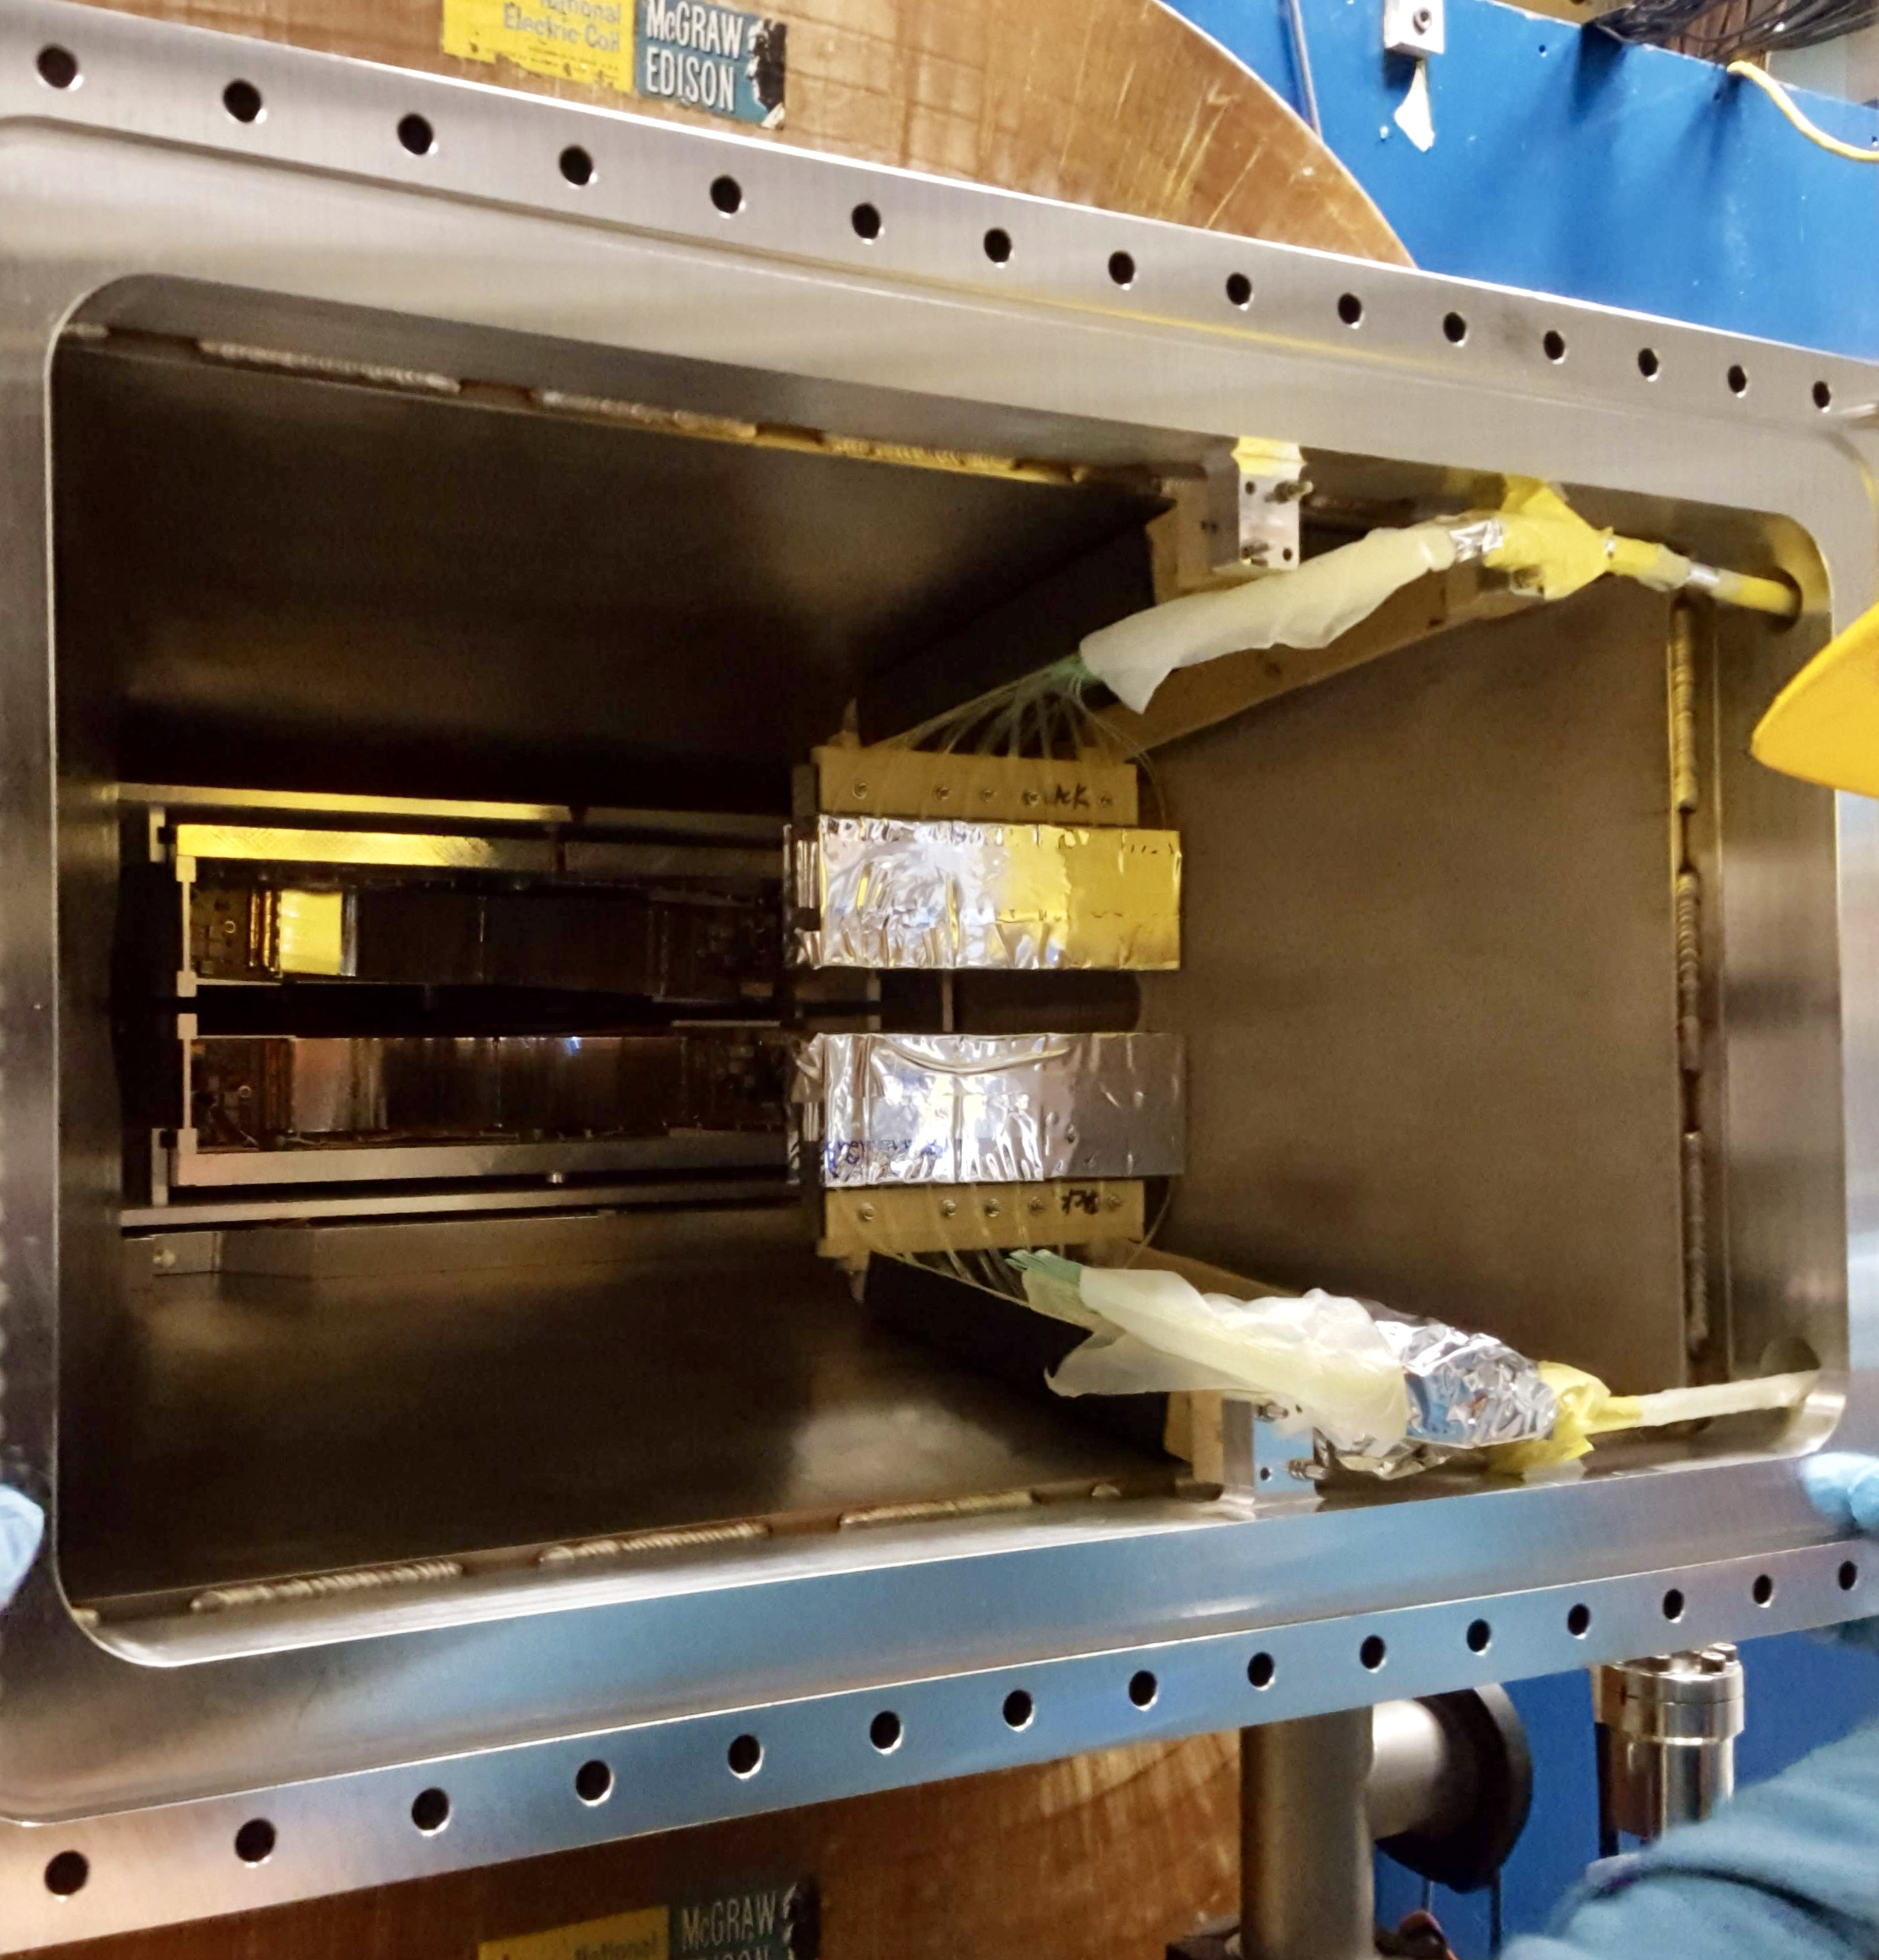
\includegraphics[width=0.45\textwidth]{figs/upgrades/Hodo_2.jpeg}
    \caption{Left: A schematic of the Ecal showing the side in which positrons trigger. The positron trigger will recover events in which the electron falls in the gap. Right: A picture of the hodoscope which is located in the vacuum chamber behind layer 6 of the SVT and in front of the Ecal, but only on the positron side. Ecal-hodoscope matching enables a positron-only trigger with rates that are manageable for the DAQ.}
    \label{fig:positrigger}
\end{figure}

In order to test the potential improvements of these upgrades, simulations were performed using an upgraded detector model with a 1.06 GeV beam. This beam energy was chosen because the analysis for the 2015 Engineering Run at 1.06 GeV was advanced at the time of these simulations and a well-understood benchmark was needed. The initial simulations presented here do not include the hodoscope which adds an additional factor of $\sim$2 to the signal yield. The goal of these simulations is to obtain the number of $\aprime$s in a near-zero background region, and determine the experiment's reach. %hence a projected sensitivity.

In order to obtain this reach estimate, the acceptance of displaced $\aprime$s, a well-defined signal region, and an overall normalization are all needed. From the simulations, the acceptance as a function of $z$ for a displaced 40 MeV $\aprime$ is shown in Fig. \ref{fig:L0eff} and Fig. \ref{fig:40MeVeff}. The signal region is defined by projecting a $z_{cut}$ utilizing the same methods of background fitting discussed in Sec. \ref{sec:tailfits}. A comparison of the $z_{cut}$ between the nominal detector and the L0 upgraded detector at several different luminosities is shown in Fig. \ref{fig:L0zcut}. Since $z_{cut}$ scales approximately with vertex resolution, $z_{cut}$ is reduced by a factor of two. And since the signal shapes are exponential in $z$, this additional signal region significantly closer to the target dramatically increases the expected signal yield.\footnote{When requiring layer 0 hits for both $\epem$ particles, the geometrical acceptance drops off earlier in the upgraded detector than the nominal detector. However, since the signal shape is exponential, the signal gain from the more optimal $z_{cut}$ far outweighs the signal loss due to acceptance. In addition, adding the L0L1 and L1L1 mutually exclusive categories nearly recovers this loss as shown in Fig. \ref{fig:40MeVeff}.}

Finally, the overall normalization was found by using the radiative fraction from the ratio of the event-weighted generator-level cross-sections of trident and WAB processes and multiplying by the number of $\epem$ pairs in a small mass window as described in Sec. \ref{sec:radfrac}. After using this number and Eq. \ref{eqn:signal_yield} to compute the number of expected $\aprime$ events, the projected sensitivity is derived by drawing a contour at 2.3 expected signal events. This contour is shown in Fig. \ref{fig:L0projections}. The contours are drawn for four weeks of continuous beam (reach is not expected in either detector configuration for the 2015 Engineering Run luminosity of 1.7 days of beam). The contour for the nominal detector is not drawn since the sensitivity is expected to begin at about 10 weeks.

\begin{figure}
    \centering
    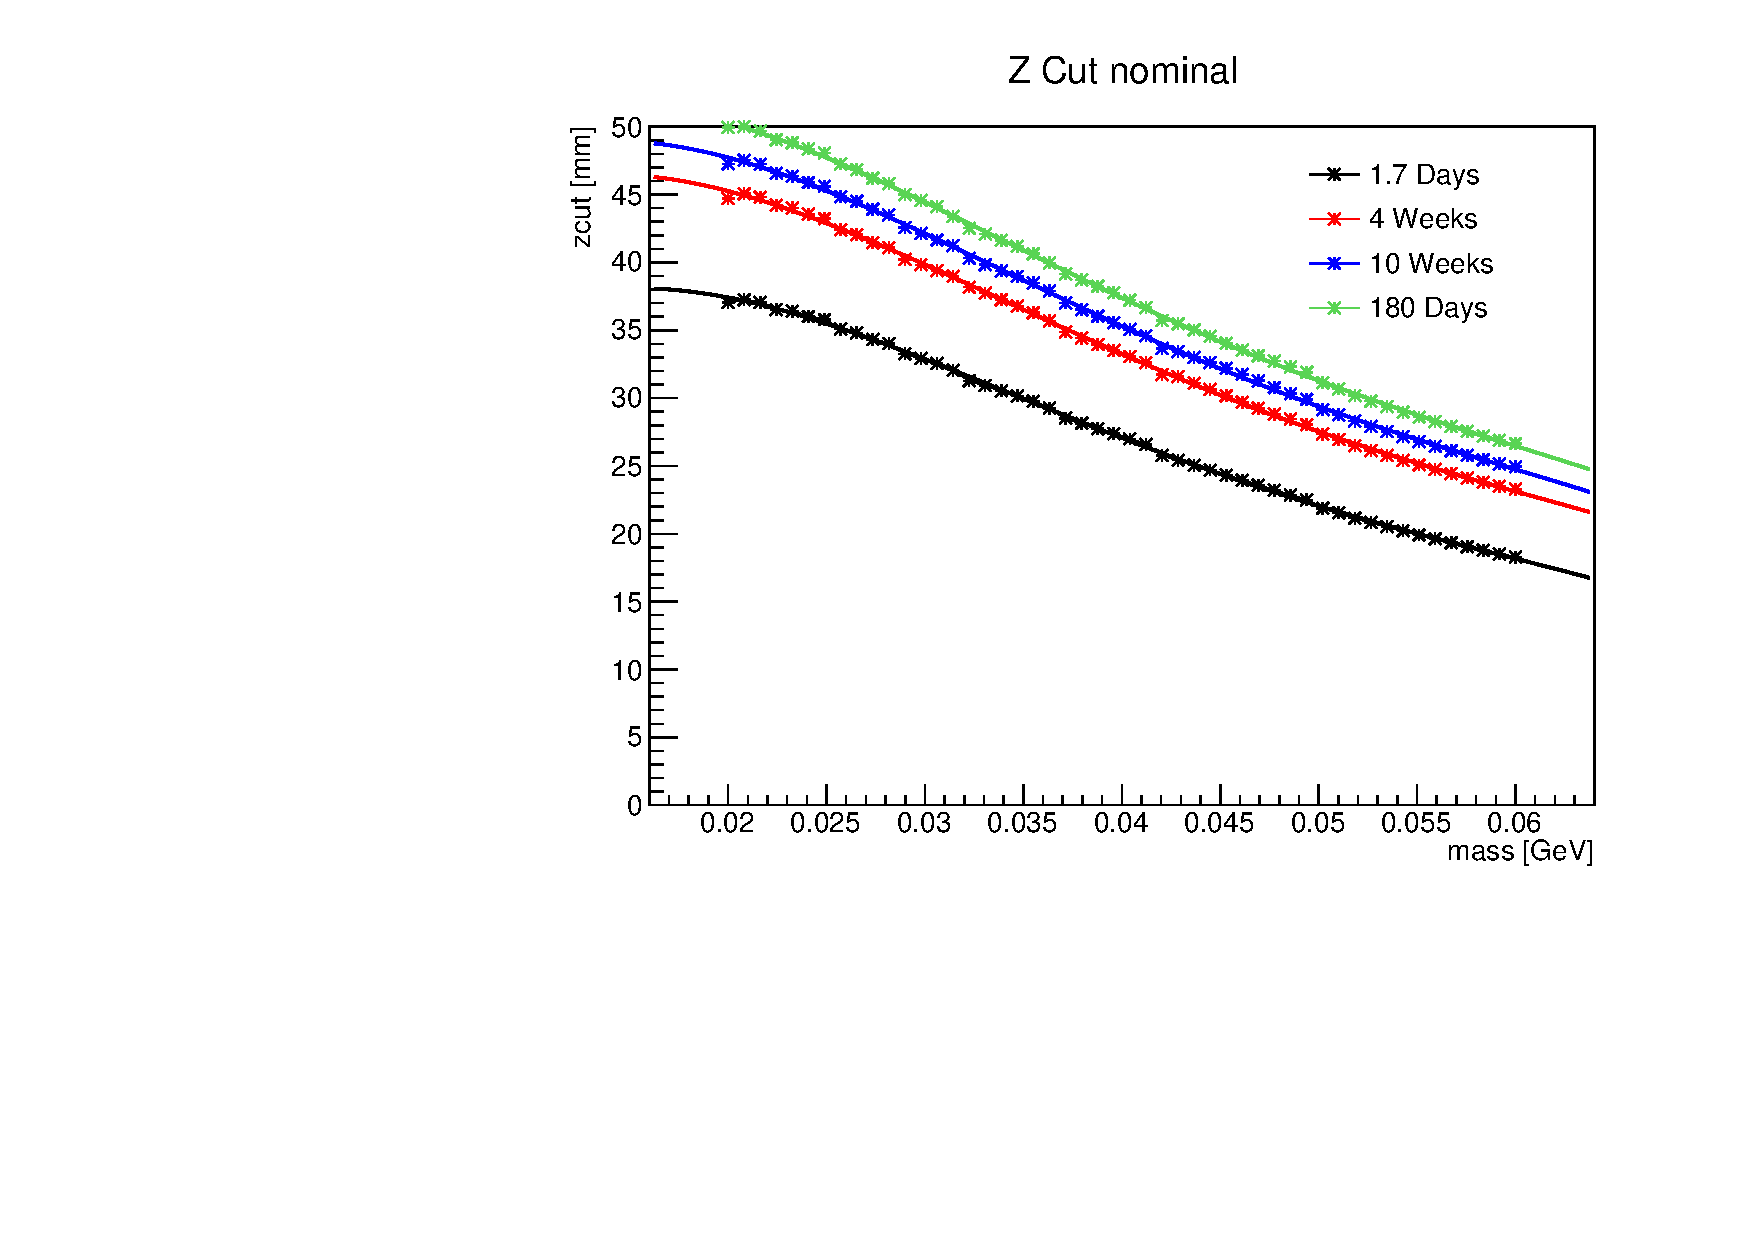
\includegraphics[width=0.45\textwidth]{figs/upgrades/zcut_nominal.pdf}
    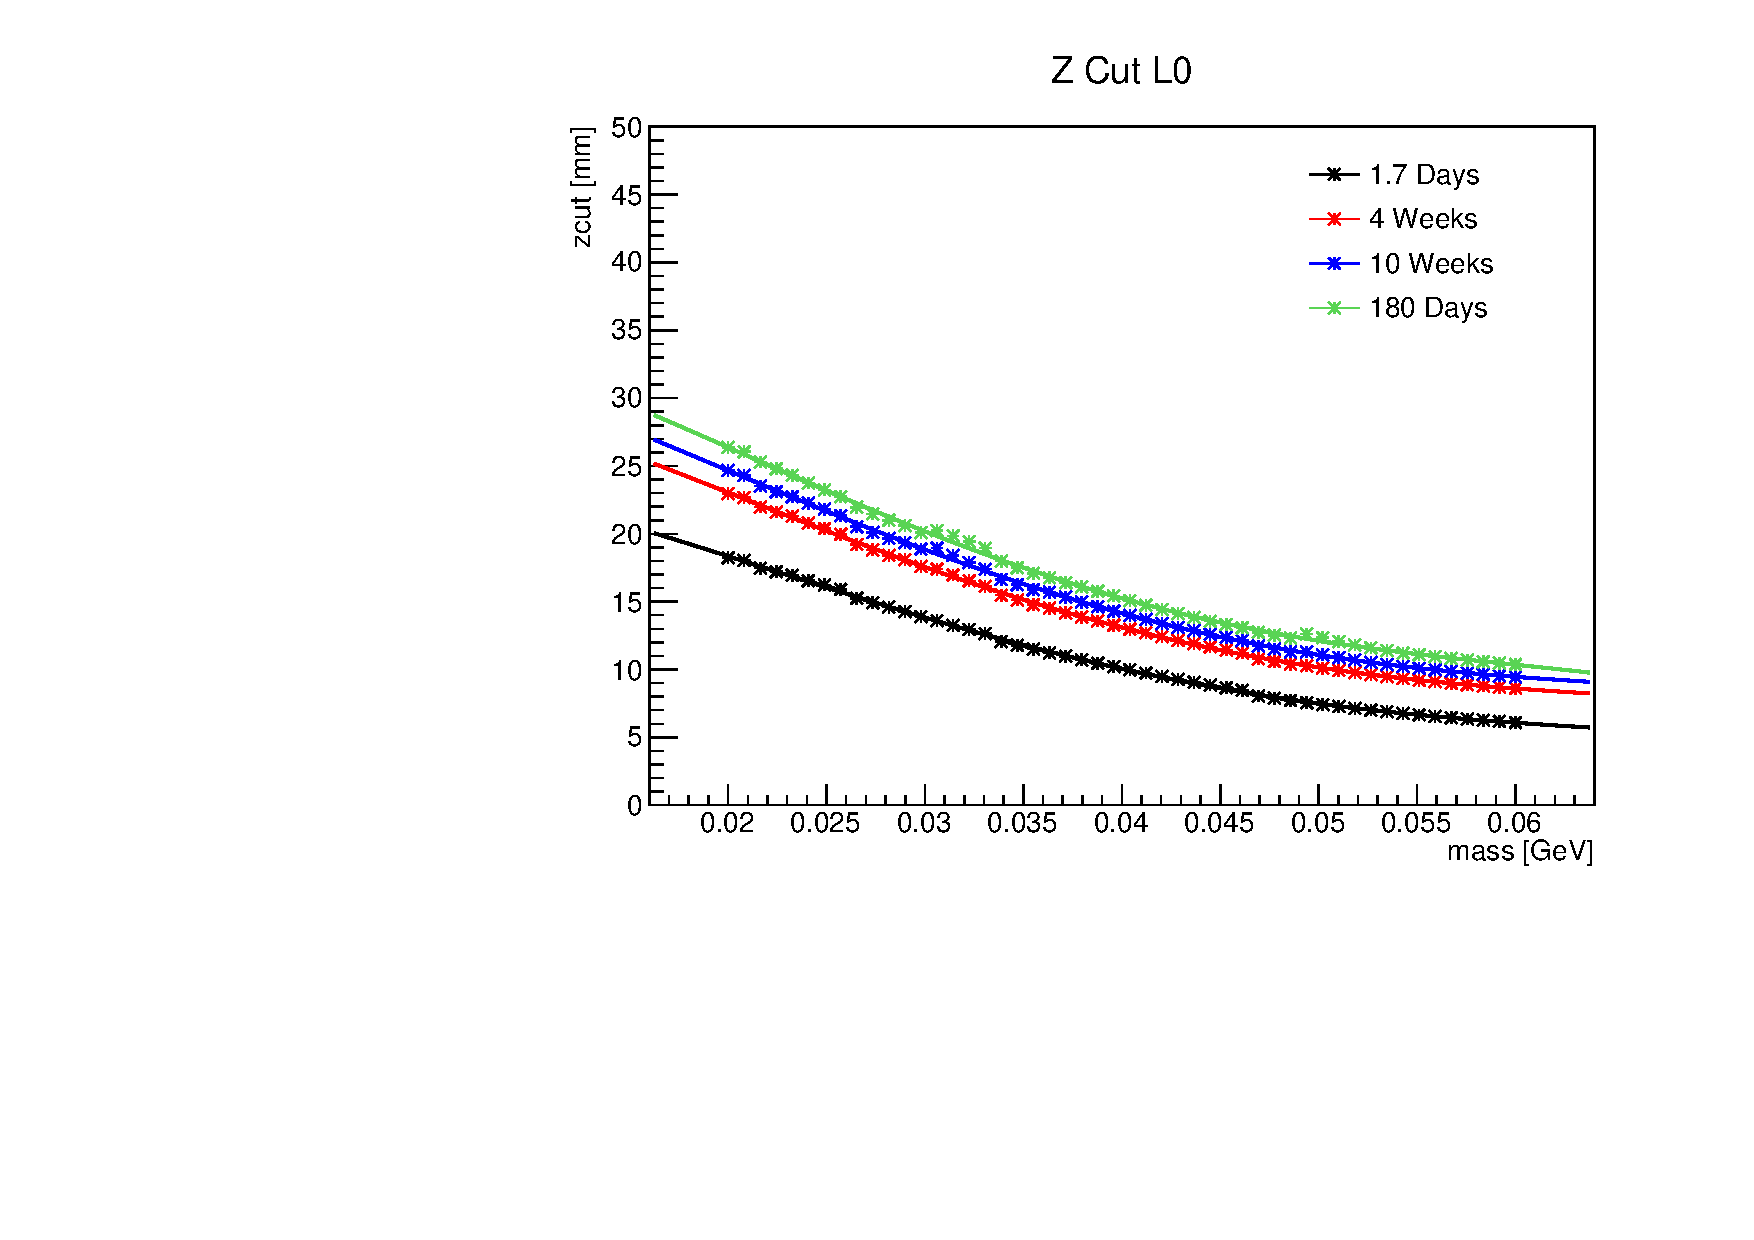
\includegraphics[width=0.45\textwidth]{figs/upgrades/zcut_L0.pdf}
    \caption{A comparison of the $z_{cut}$ for several different luminosities (1.7 days, 4 weeks, 10 weeks, and 180 days) for Left: the nominal detector and Right: the upgraded L0 detector. The improvement in $z_{cut}$ by a factor of $\sim 2$ for the L0 detector is a measure of the the improvement in the signal yield. $z_{cut}$ increases with luminosity since the overall scale in the background fit also increases with luminosity, and the point beyond which 0.5 background events is expected is pushed to higher $z$.}
    \label{fig:L0zcut}
\end{figure}

\begin{figure}
    \centering
    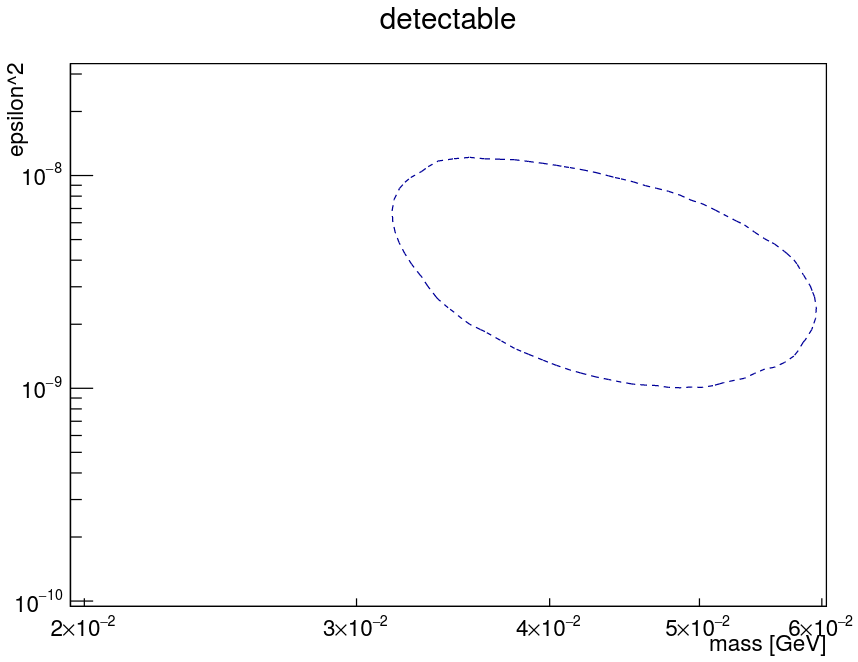
\includegraphics[width=0.5\textwidth]{figs/upgrades/L0_4weeks_detectable.png}
    \caption{The estimated contour for excluding $\aprime$ production in the mass-$\epsilon^2$ plane from early simulations for the upgraded L0 detector assuming 4 weeks of a continuous 1.06 GeV beam. The contour is drawn at 2.3 expected events and assumes layer 0 hits for both $\epem$ particles (L0L0).}
    \label{fig:L0projections}
\end{figure}

%\clearpage

The construction of the upgraded SVT began at SLAC in the winter of 2019. A picture of a completed L0-3 U-channel on the mechanical survey table is shown in Fig. \ref{fig:testbox}. After the mechanical survey was complete, each upgraded U-channel was placed in a test box for testing of the DAQ as shown in Fig. \ref{fig:testbox}. These boxes were weather-sealed and pumped continuously with dry air to allow for cooling without condensation. The cooling system was hooked up to the nominal SVT cooling system. The humidity was monitored with humidity sensors and an Arduino-based readout system with a Twitter-based alert system as shown in Fig. \ref{fig:twitter} \cite{hpstweet2019}.

After testing at SLAC, the upgraded U-channels were shipped to Jefferson Laboratory and installed in the HPS SVT box inside the analyzing magnet. The installation was performed in May and June of 2019, in time for the middle of June start of the run. A picture of the completely installed upgraded U-channels (without the target) for both the ``open'' and ``closed'' SVT configurations is shown in Fig. \ref{fig:SVTview}.

\begin{figure}
    \centering
    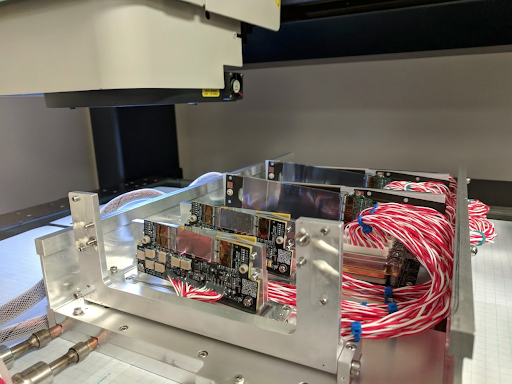
\includegraphics[width=0.5\textwidth]{figs/upgrades/U0_3.png}
    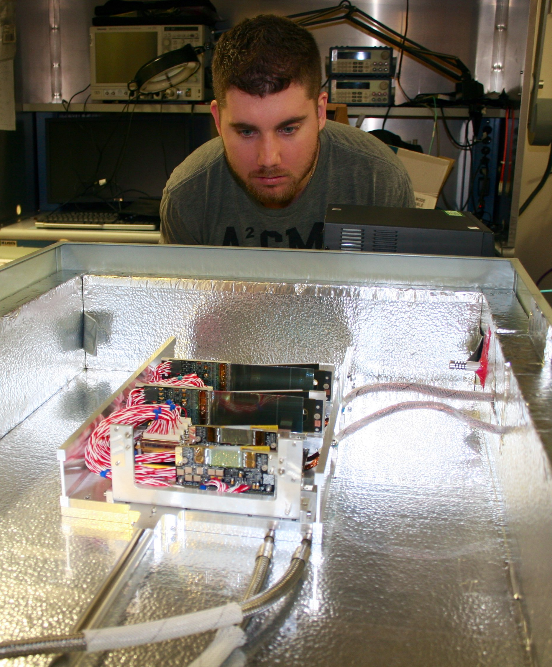
\includegraphics[width=0.5\textwidth]{figs/upgrades/test_box.png}
    \caption{Left: A picture of an L0-3 U-channel on top of the mechanical survey table. Right: A graduate student peers over an L0-3 U-channel inside a test box at SLAC that was used for DAQ testing.}
    \label{fig:testbox}
\end{figure}

\begin{figure}
    \centering
    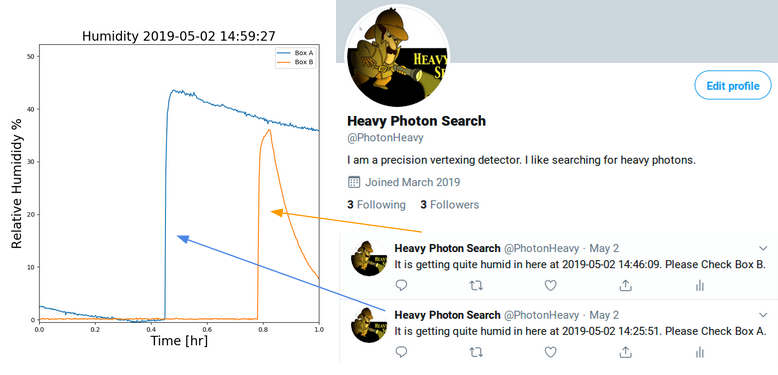
\includegraphics[width=0.75\textwidth]{figs/upgrades/twitter.png}
    \caption{The upgraded U-channels were each placed in a test box at SLAC for DAQ testing. Since each box must be cooled and fed dry air, humidity monitoring is needed. Each box contained a humidity sensor which was readout via an Arduino and connected to a Twitter-based alert system. This picture shows an example of a sudden increase in humidity in both test boxes which was immediately followed by an alert tweet. In other words, someone opened the test boxes \cite{hpstweet2019}.}
    \label{fig:twitter}
\end{figure}

\begin{figure}
    \centering
    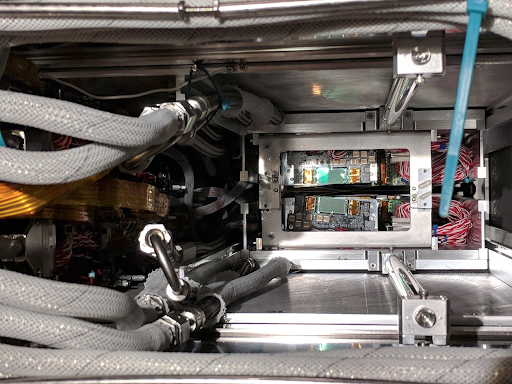
\includegraphics[width=0.45\textwidth]{figs/upgrades/SVT_L0_open.png}
    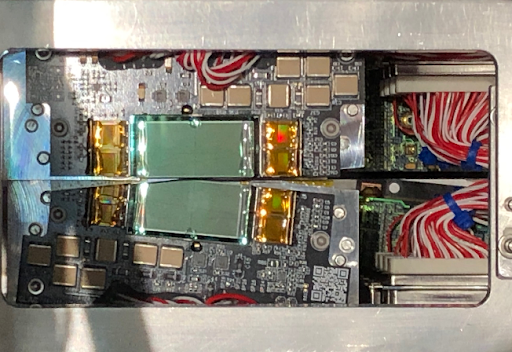
\includegraphics[width=0.45\textwidth]{figs/upgrades/SVT_L0_closed.png}
    \caption{Left: A beam's-eye view of the installed L0 sensors inside the vacuum chamber. This is in the ``open'' configuration in which the sensors are far from the beam plane ($\sim 10$ mm) so that the beam can be tuned without damaging sensors. Right: A zoomed in version in the ``closed'' (or operating) configuration where the L0 axial sensors are 500 $\mu$m from the beam plane. }
    \label{fig:SVTview}
\end{figure}

\clearpage

%\section{Upgrade Performance}\label{sec:upgradeperformance}

\section{Preliminary Upgrade Performance \& Reach Estimates}\label{sec:2019data}

Beam commissioning for the 2019 Physics Run began in the middle of June in 2019. This was the first simultaneous running of Hall A, Hall B, and Hall C in the 12 GeV era (where each hall requested unique beam requirements) which resulted in difficulty in delivering quality beam for several weeks. In addition, several issues from HPS interrupted data taking. First, a site-wide power outage due to a storm caused a trip in the analyzing magnet which subsequently shifted the bottom U-channel by more than 10 mm. It is assumed that currents induced by the rapidly changing magnetic flux induced currents in the SVT structures which led to large forces on the SVT. Second, significant radiation damage from frequent beam tuning  and poor beam quality in Hall B caused significant damage to the front end electronics, making some channels barely usable. Third, a broken grounding wire for the target (which was not identified until the vacuum chamber was closed) caused charge to accumulate and then frequently discharge, resulting in bursts of electronic noise and DAQ failures. A summary timeline of important events over the 2019 Physics Run is shown in \ref{fig:2019timeline}.

\begin{figure}
    \centering
    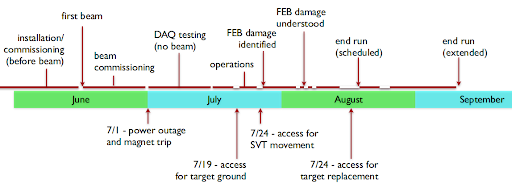
\includegraphics[width=0.75\textwidth]{figs/upgrades/2019_timeline.png}
    \caption{The approximate timeline for the major events that occurred over the course of the 2019 Physics Run. The first beam was delivered to the Hall B in the middle of June. Due to issues over the course of the run, the run was extended from the end of August to the middle of September.}
    \label{fig:2019timeline}
\end{figure}

Despite significant issues, excellent beam conditions were achieved at the end of July. An SVT wire scan of one of the first beam profiles used for physics data taking is shown in Fig. \ref{fig:beam2019}. This beam had a $\sim 22 \ \mu$m spot size in $y$ and was within $\sim 50 \ \mu$m of the center of the detector. And once beam quality was consistent, data was efficiently collected. In total, 110 $pb^{-1}$ of luminosity was accumulated (equivalent to about $\sim$2 weeks of continuous beam) as shown in Fig. \ref{fig:data2019}. This is about three times the total run time of the 2016 Engineering Run.

\begin{figure}
    \centering
    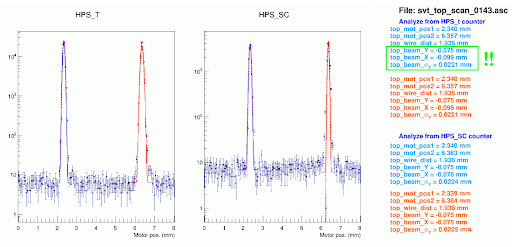
\includegraphics[width=0.85\textwidth]{figs/upgrades/2019_beam.png}
    \caption{A measurement of the beam profile using the SVT scan wires showing a beam width of 22 $\mu$m in $y$ within 50 $\mu$m of the center of the detector. This is a high-quality beam was the first successful beam for HPS with simultaneous operations of Hall A, Hall B, and Hall C in the 12 GeV era (upgraded CEBAF as described in Sec. \ref{sec:cebaf}).}
    \label{fig:beam2019}
\end{figure}

\begin{figure}
    \centering
    %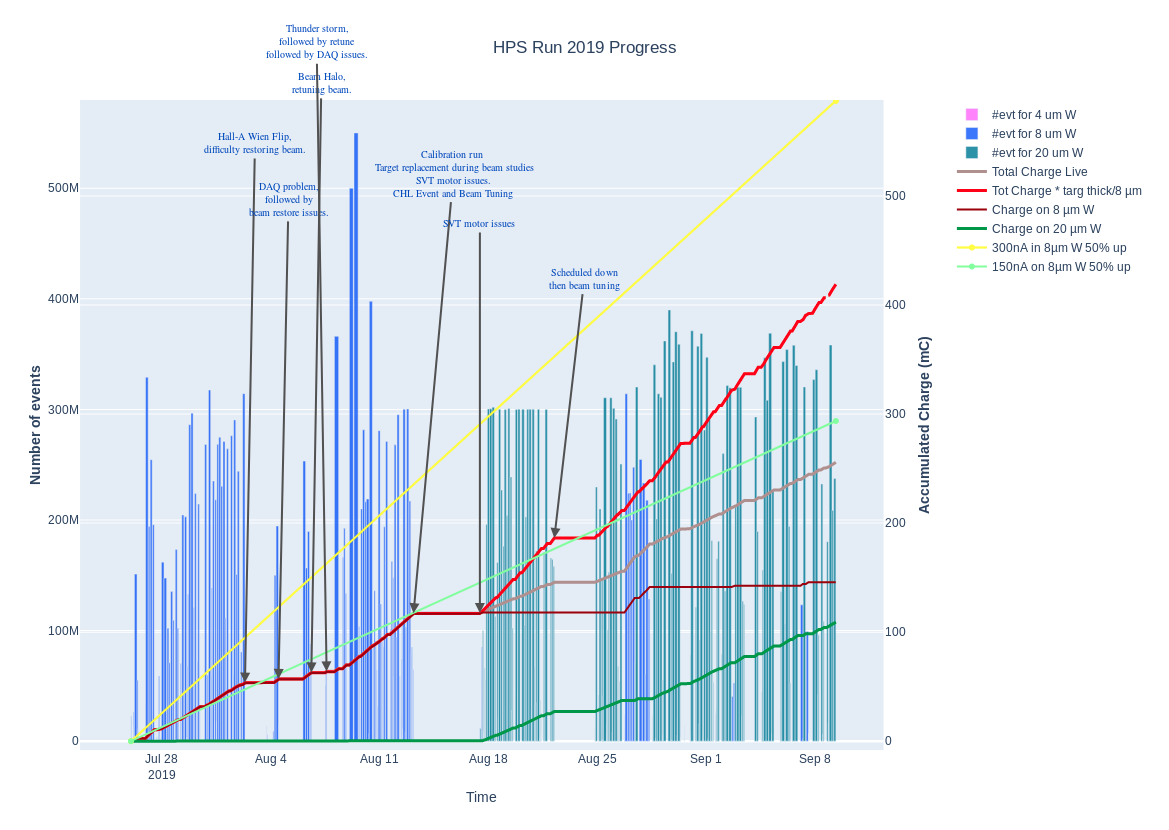
\includegraphics[width=0.5\textwidth]{figs/upgrades/data_2019.png}
    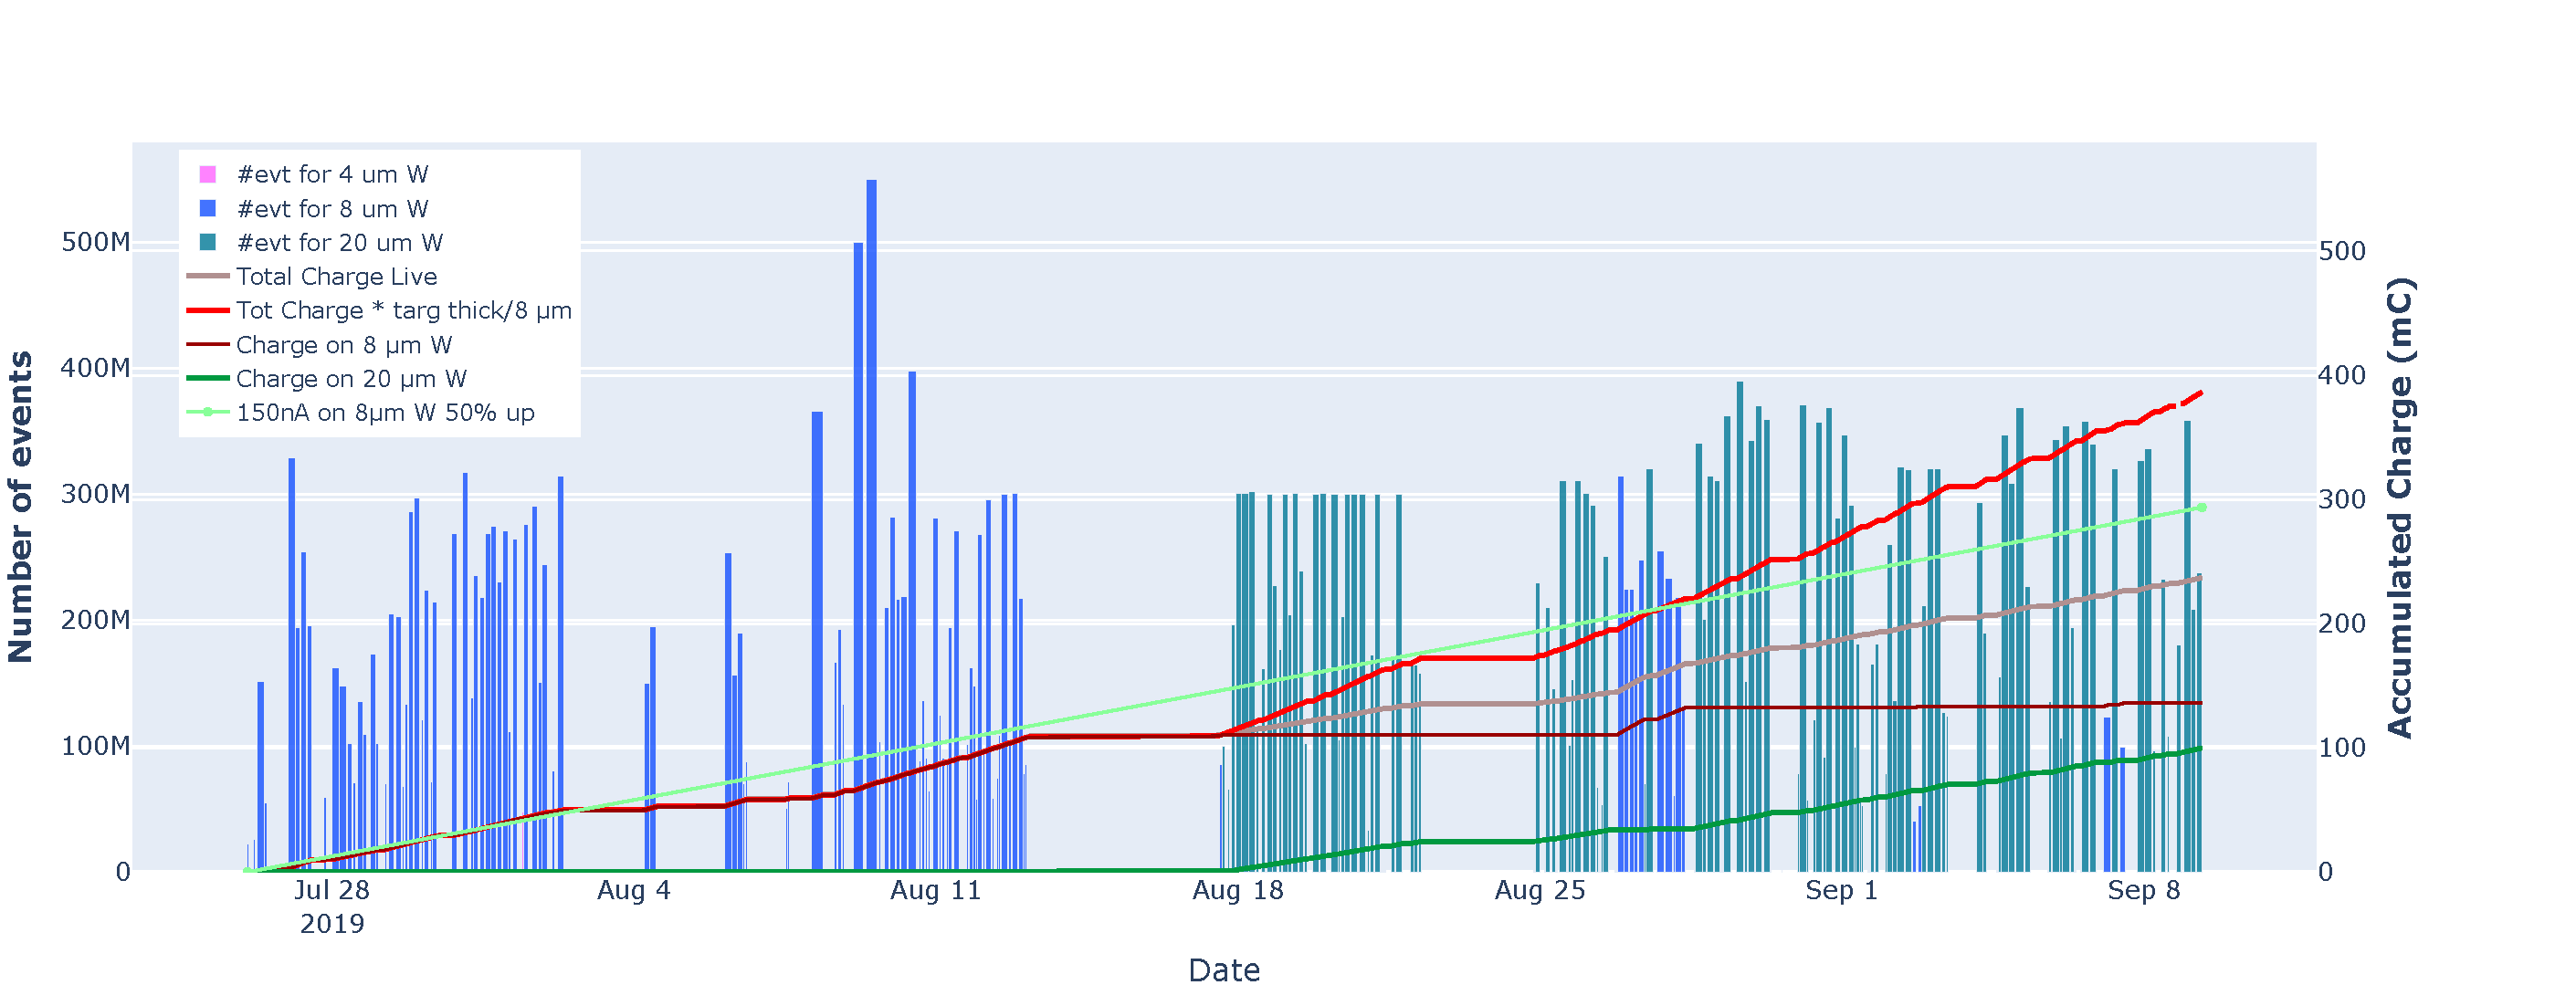
\includegraphics[width=1.0\textwidth]{figs/upgrades/HPSRun2019_progress-1.pdf}
    \caption{Accumulated charge over the course of the 2019 Physics Run. The red line is re-scaled to the luminosity-equivalent total charge from an 8 $\mu$m thick target since the target configuration was changed several times over the course of the run.}
    \label{fig:data2019}
\end{figure}

In order to prove the effectiveness of the upgrades, an improved vertex resolution in agreement with MC and an $\epem$ rate increase from the hodoscope and positron-only trigger must be shown. The preliminary results from the 2019 Physics Run shows nearly a 1 mm vertex resolution in the mass range of interest which is about $\sim$25\% worse than current MC predictions. However, this is far from the final tracker alignment and as the alignment converges on its optimal configuration, the vertex resolution will improve. Evaluating the effectiveness of moving L1-L3 closer to the beam plane is in process.

In terms of the effectiveness of the hodoscope, one can compare the total $\epem$ rate with the fraction of the $\epem$ rate that does not contain a match with an electron-side cluster. Preliminary results shown in Fig. \ref{fig:prelimdata2019} show an increase in rate of about $\sim 30$\% in the momentum sum signal region. However, these preliminary results depend on the finding of an electron track. Track finding is expected to improve as both tracker alignment improves and as a Kalman Filter track finding algorithm is implemented.\footnote{For the 2015 and 2016 Engineering Runs, the SeedTracker algorithm was used for track finding as described in Sec. \ref{sec:tracking}. However, several sensors were turned off over the course of the 2019 Physics Run due to issues with both the sensors and FEBs. SeedTracker relies on the use of 3D hits, thus incorporating a Kalman Filter which performs track finding at the strip hit level will recover a significant number of tracks.}

\begin{figure}
    \centering
    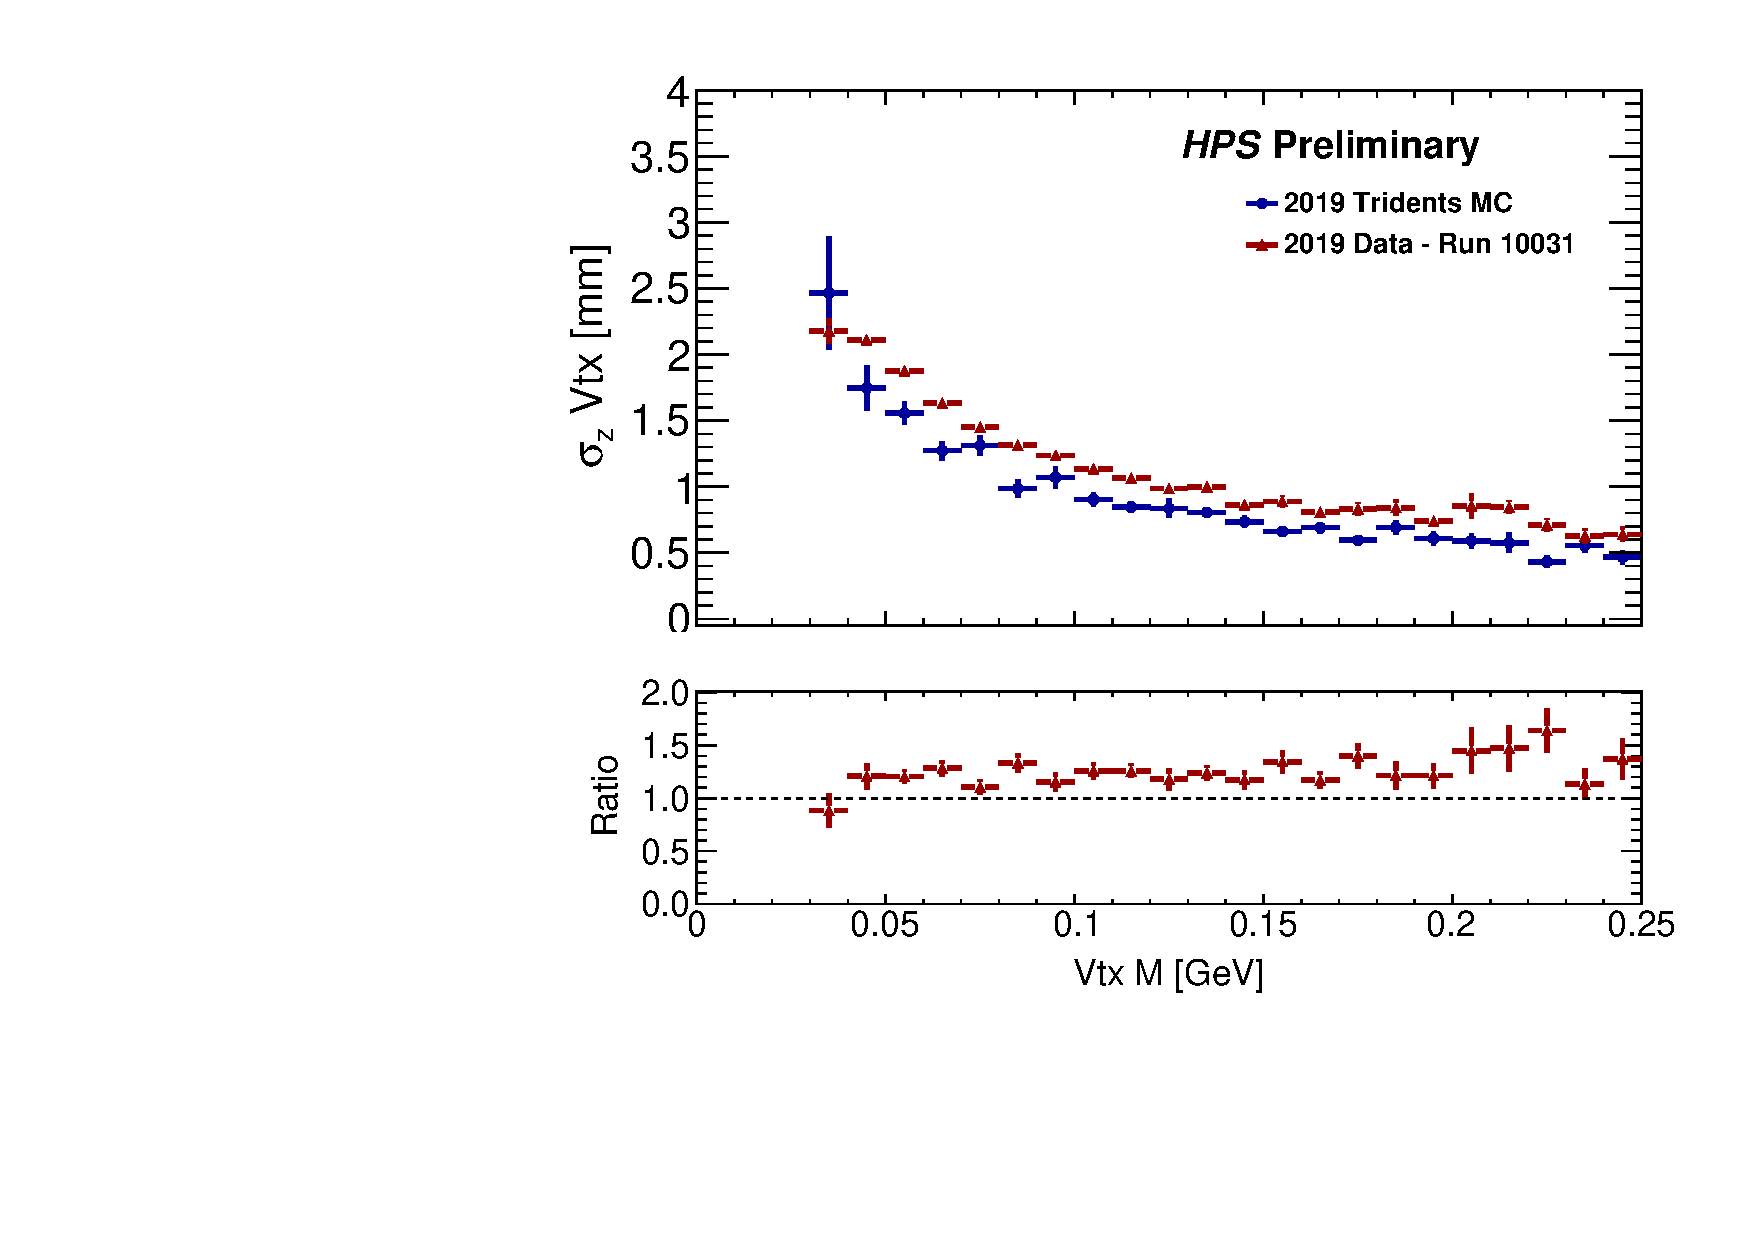
\includegraphics[width=0.45\textwidth]{figs/upgrades/vtxana_gbl_tightUncVChi2_vtx_InvM_vtx_svt_z_hh_sigma.pdf}
    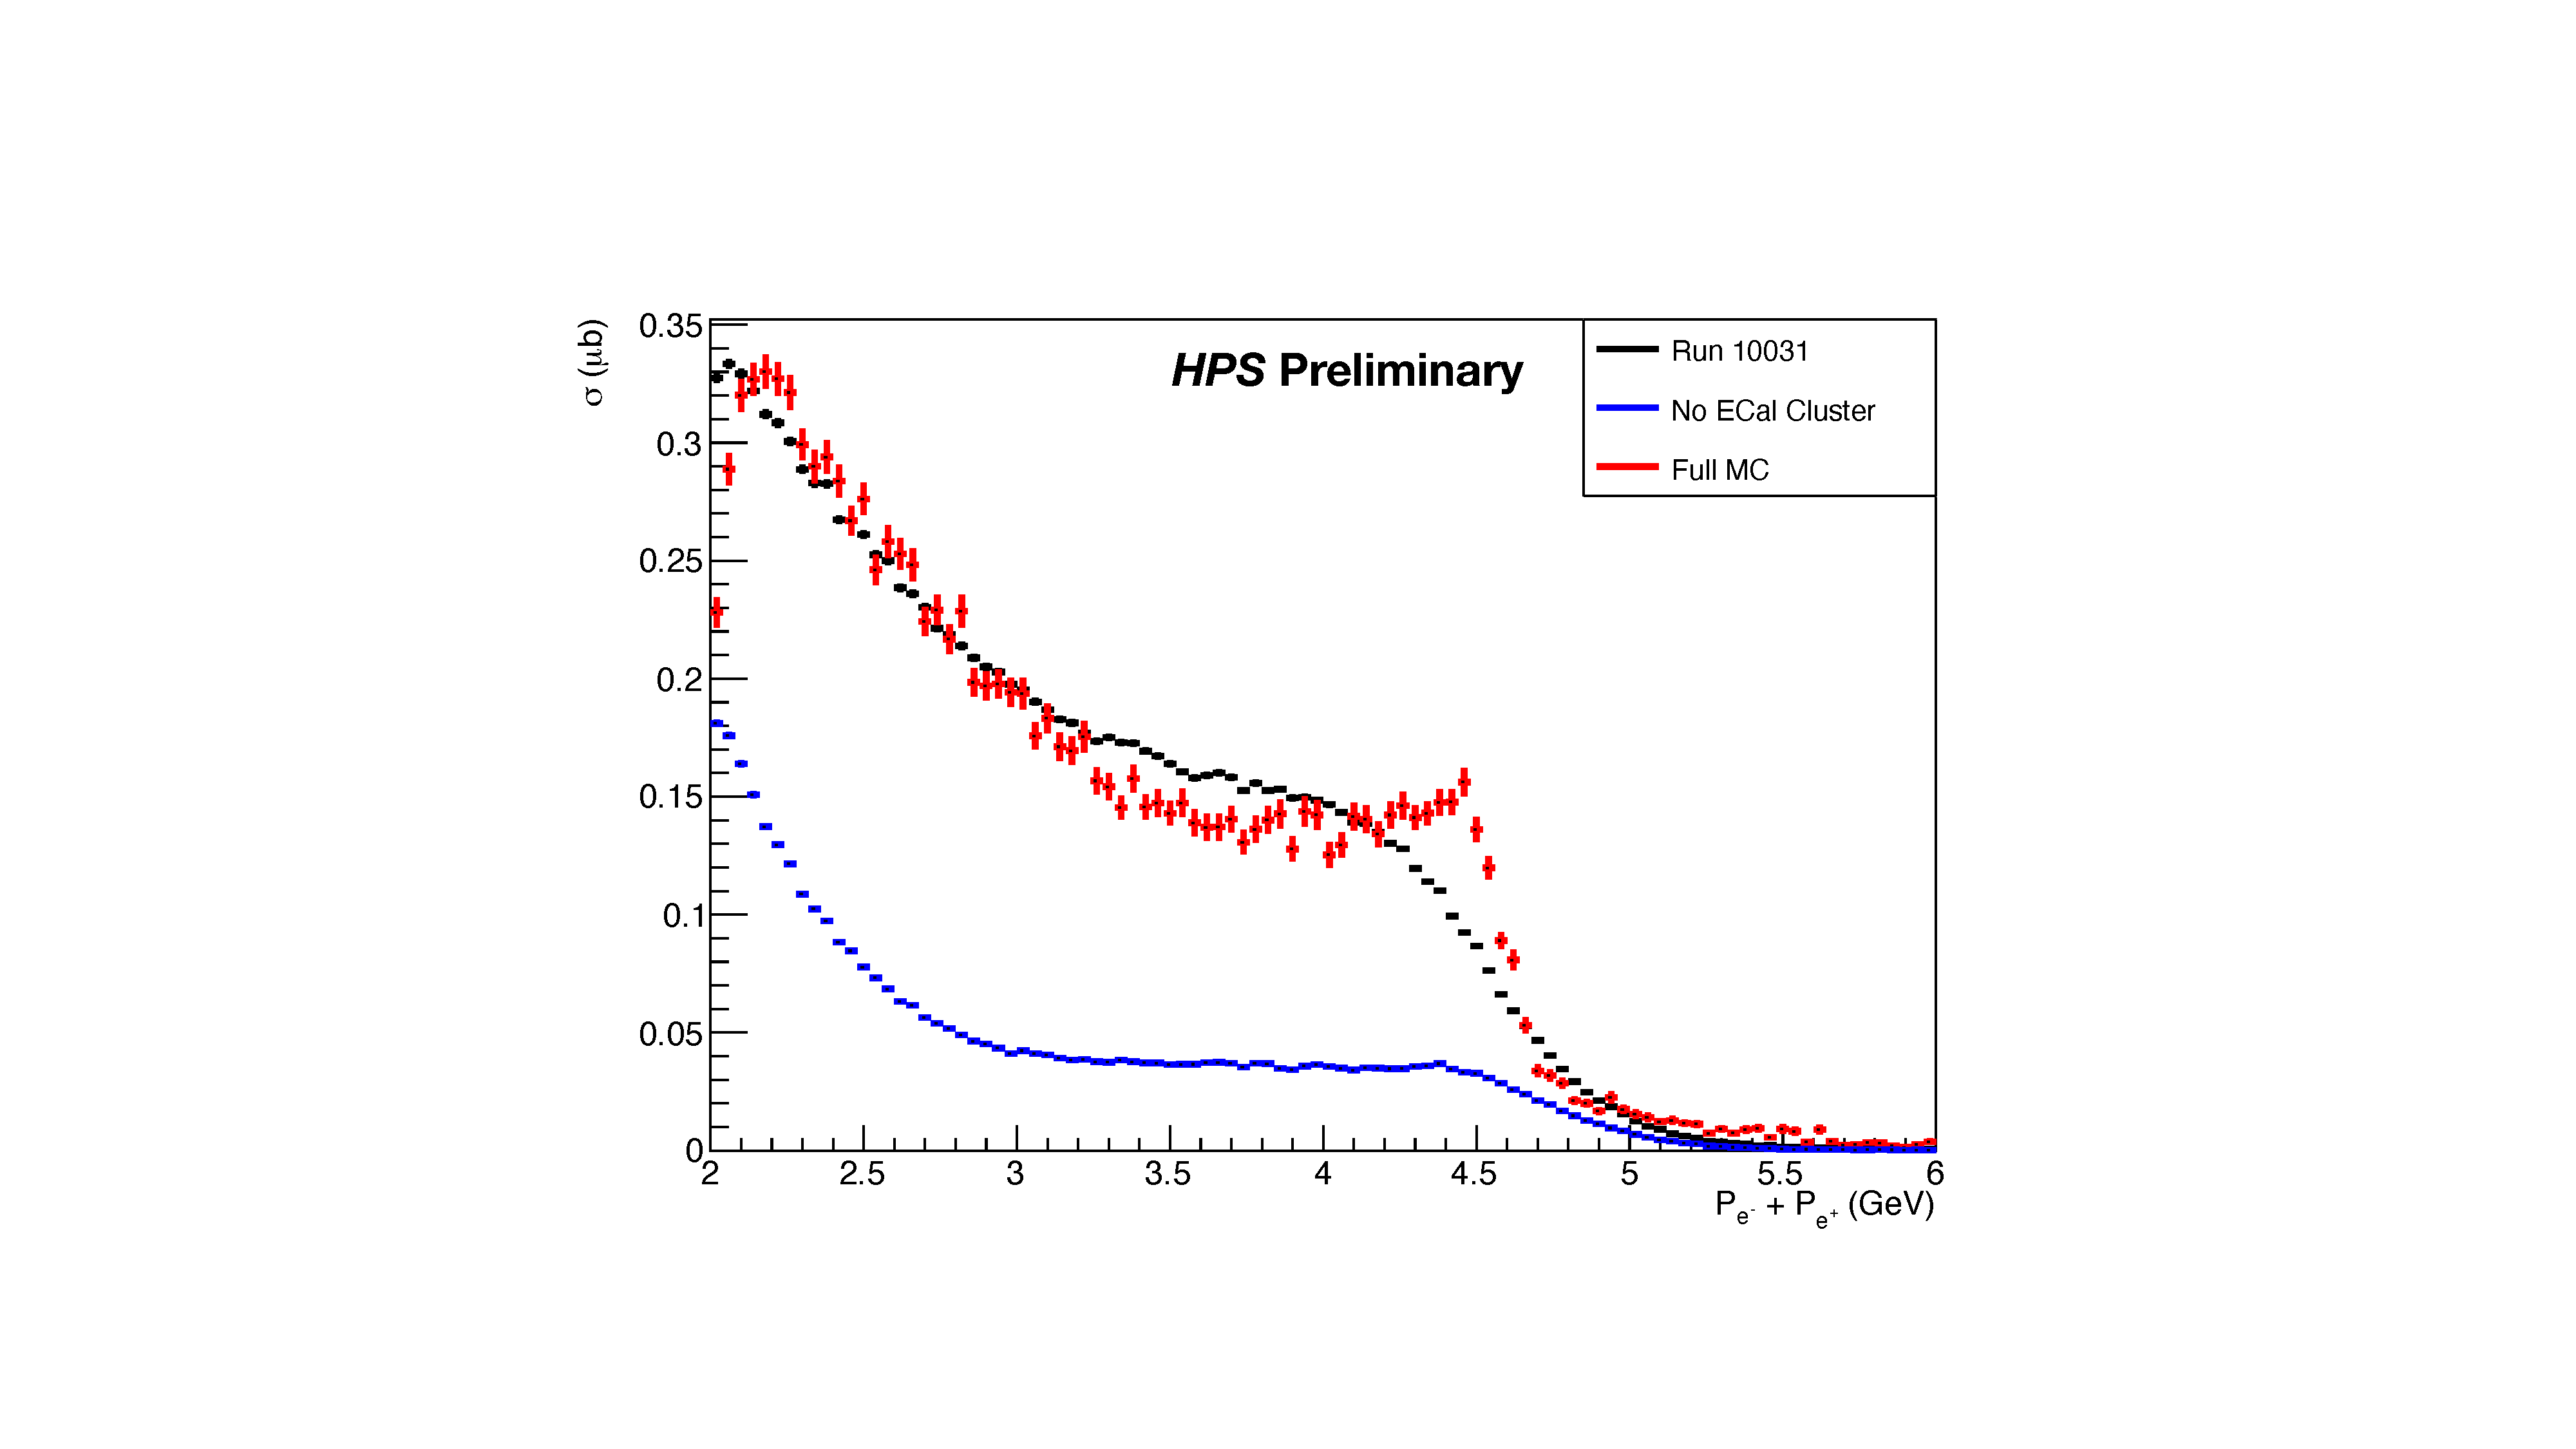
\includegraphics[width=0.45\textwidth]{figs/upgrades/psum_2019.pdf}
    \caption{Left: A comparison of the vertex resolution for data and MC for with a 4.55 GeV beam. Data is within $\sim 25$\% of MC and will improve as the tracker alignment is updated. Right: A comparison of data and MC measured cross-sections as a function of $\epem$ momentum sum. The blue line represents events in which the electron track does not match to a cluster in the Ecal. This is a measure of the effectiveness of the hodoscope which shows an increase in the rate of $\epem$ pairs by $\sim$30\% in the signal region (large momentum sum).}
    \label{fig:prelimdata2019}
\end{figure}

From the initial analysis in the data, one can project the expected sensitivity for the displaced vertexing analysis shown in Fig. \ref{fig:projections}. This projection is conservative since it requires layer 0 hits for both $\epem$ particles (L0L0). However, it is likely that adding the other mutually exclusive categories (L0L1, L1L1, etc.) to capture $\aprime$s with longer livetimes will add significance to the analysis. This is especially true in the upgraded detector since layers 1 -3 in the SVT were moved closer to the beam plane for increased $\aprime$ acceptance of further downstream decays. The projected sensitivities of these additional categories have not been explored yet.

\begin{figure}
    \centering
    %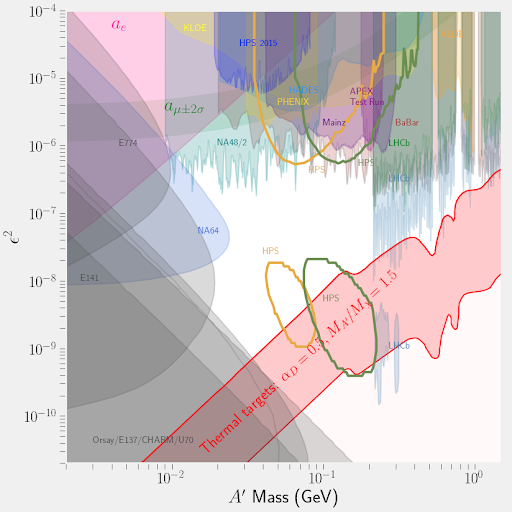
\includegraphics[width=0.5\textwidth]{figs/upgrades/hps_projections.png}
    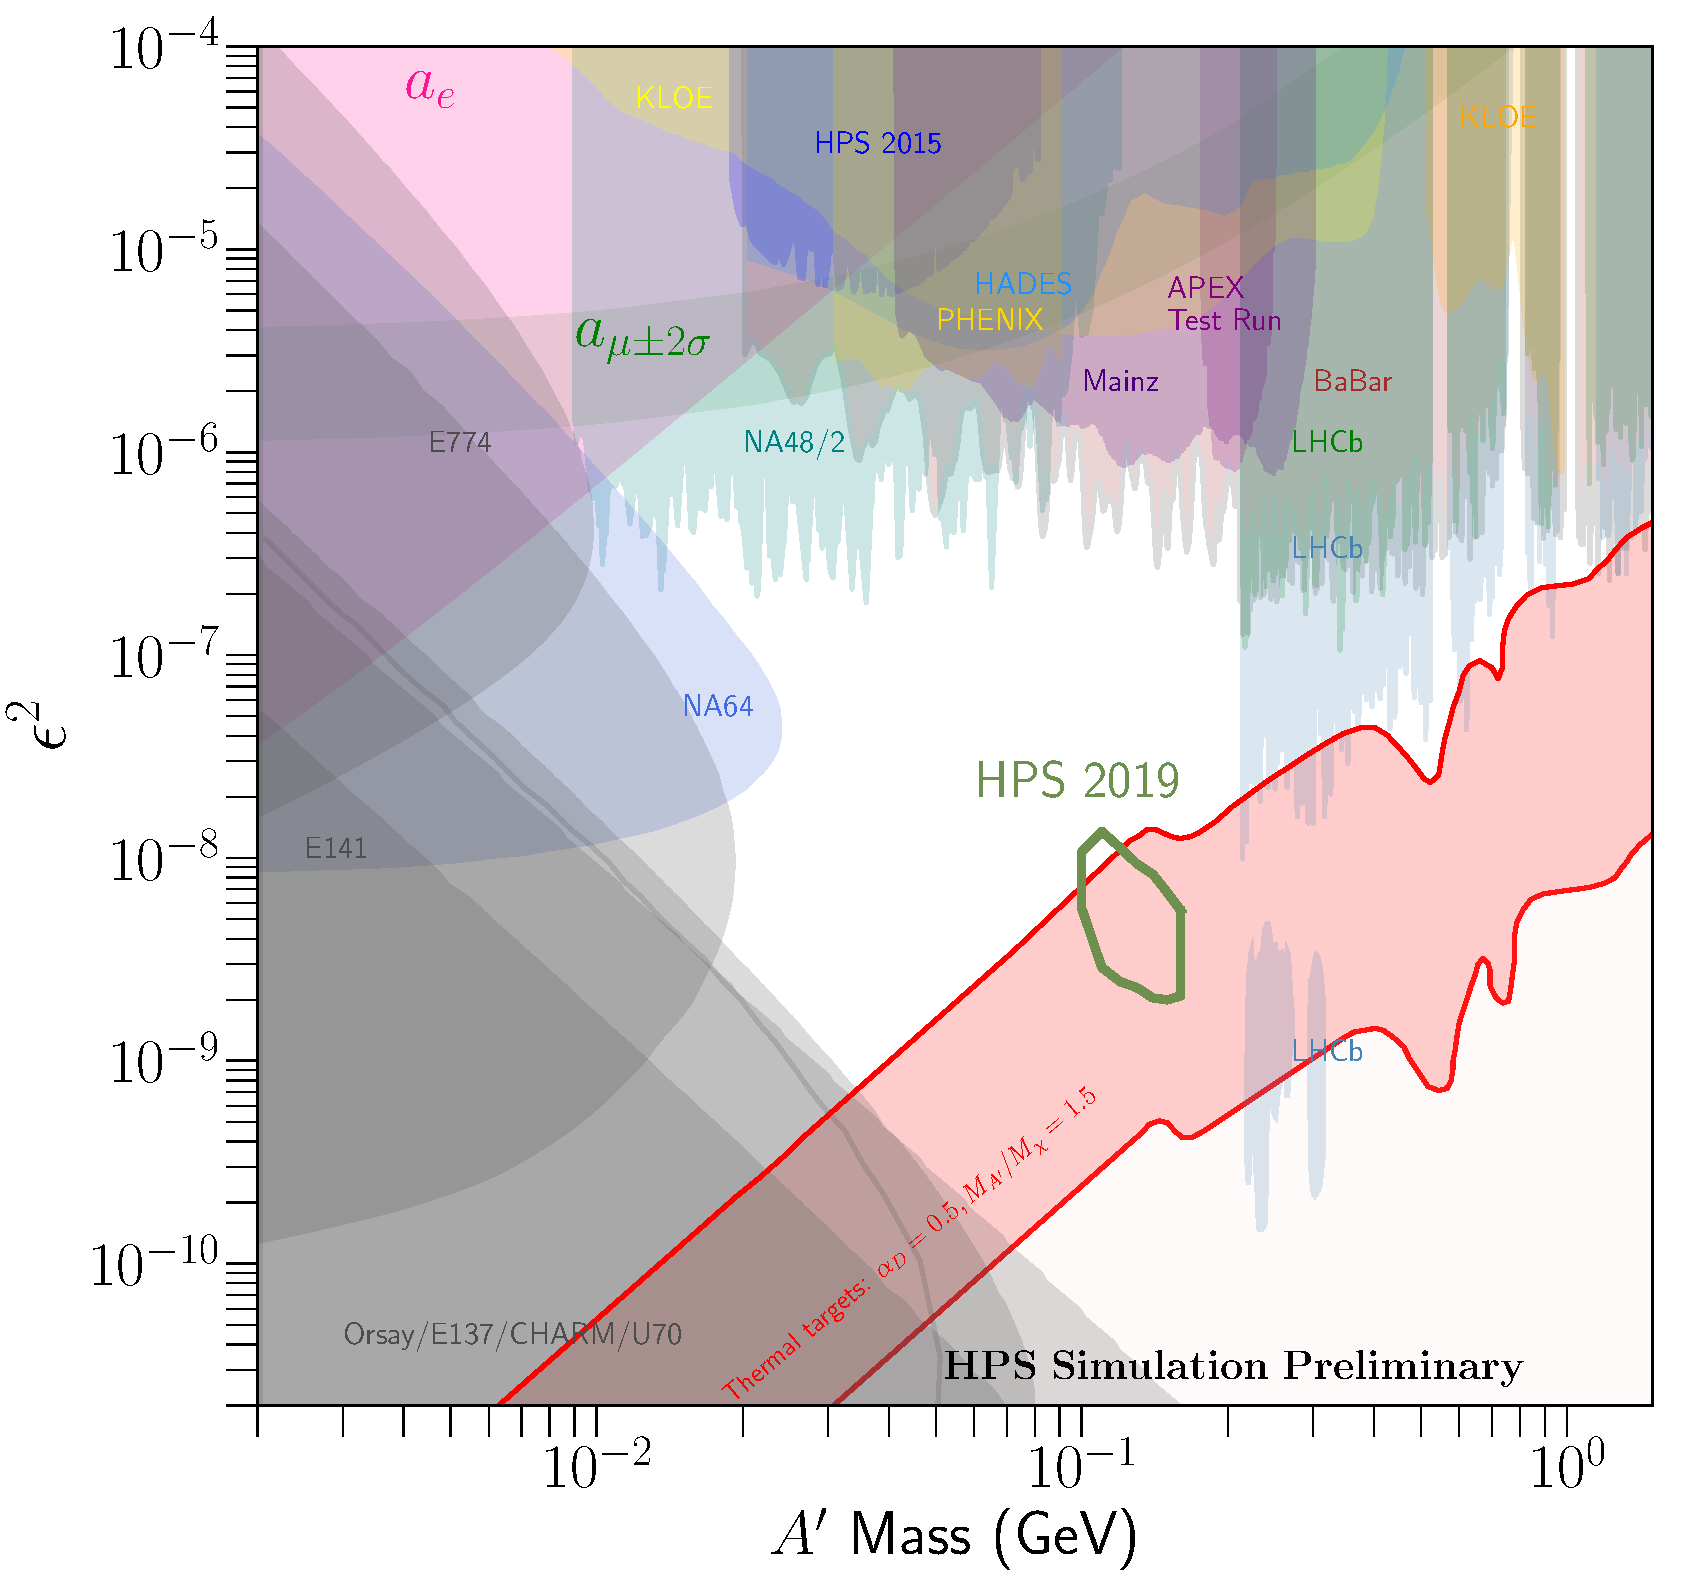
\includegraphics[width=0.65\textwidth]{figs/upgrades/reach_2019.pdf}
    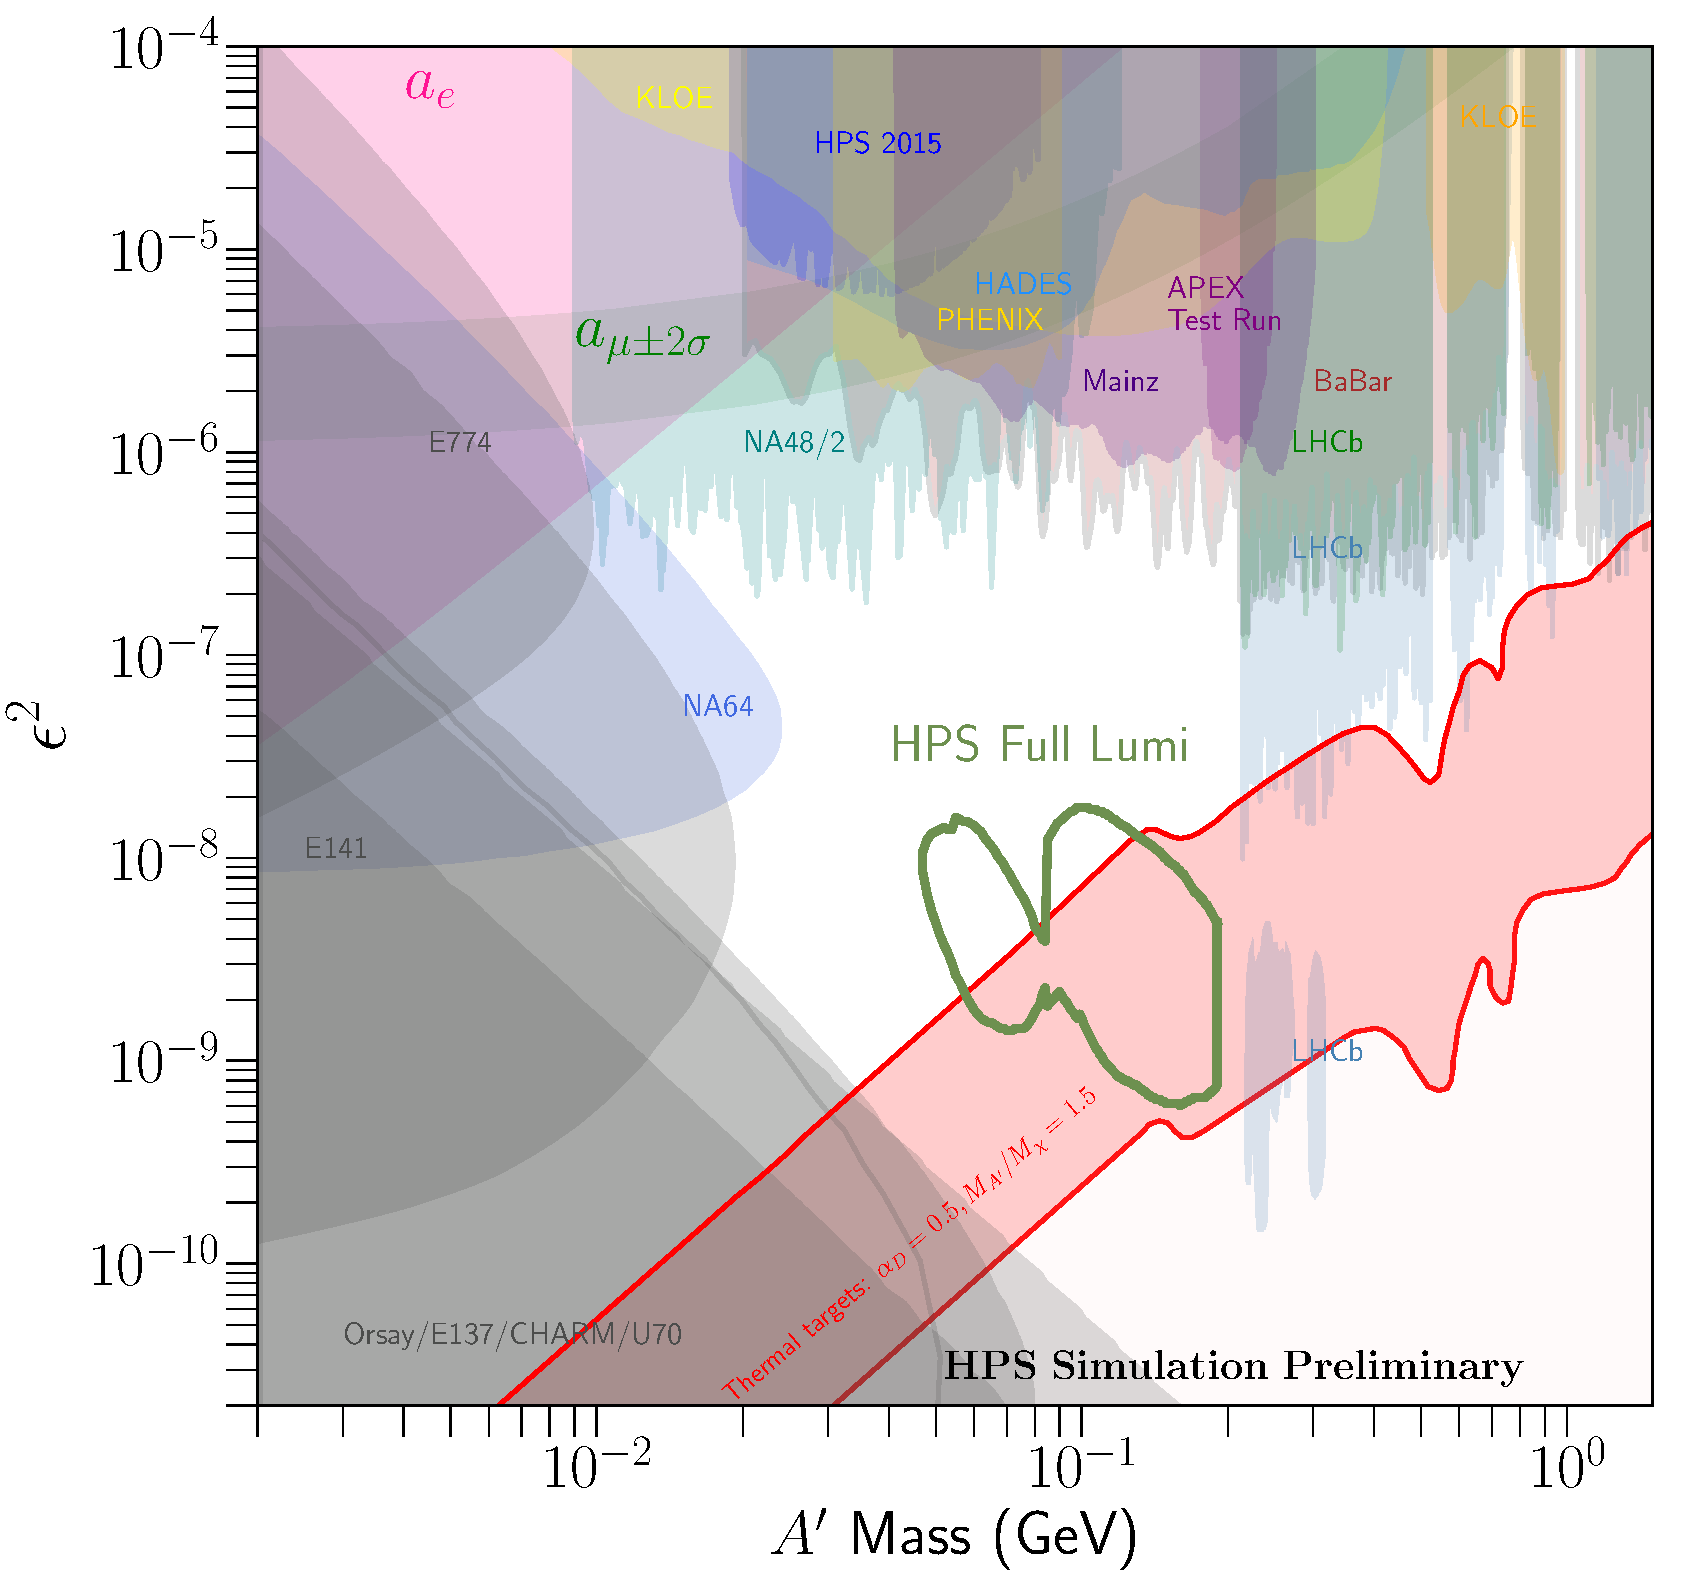
\includegraphics[width=0.65\textwidth]{figs/upgrades/reach_full_lumi.pdf}
    \caption{Top: Initial projections for the displaced vertex search from the 2019 Physics Runs with a 4.55 GeV beam. Bottom: Projections utilizing the full HPS run time of 180 days at both 4.55 GeV and 2.3 GeV. Both of these projections assume layer 0 hits for both $\epem$ particles (L0L0).}
    \label{fig:projections}
\end{figure}

\clearpage

%\section{Reach Estimates}\label{sec:futurereach}

%\clearpage

\section{Generalized Displaced Vertices}\label{sec:gen_vert}

In addition to the minimal $\aprime$ model described in Sec. \ref{sec:theory}, HPS can potentially probe any model with an electro-produced long-lived mediator that decays to $\epem$ pairs and set limits on the mass, livetime, and cross sections of long-lived particles that decay in the range $\sim$1-10 cm.

\subsection{Strongly Interacting Massive Particles (SIMPs)}\label{sec:simps}

\begin{figure}
    \centering
    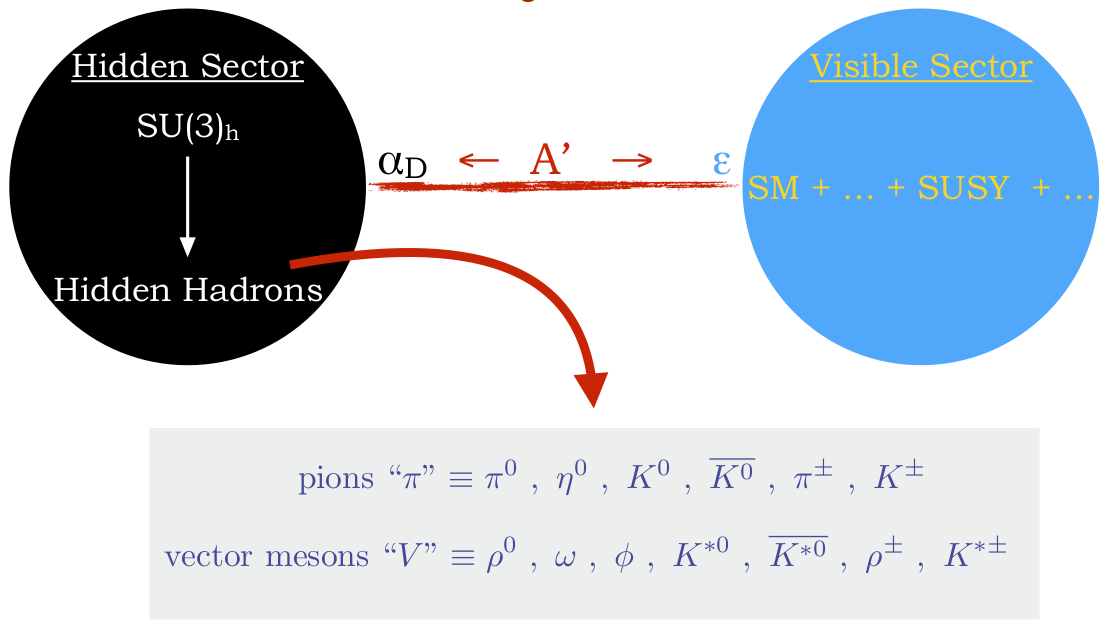
\includegraphics[width=0.85\textwidth]{figs/upgrades/su3.png}
    \caption{A hidden $SU(3)$ symmetry in a dark sector can contain hidden hadrons which include dark pions and dark vector mesons. One way for these particles to interact with SM matter is through an indirect interaction via kinetic mixing between an $\aprime$ and the SM photon as described in Sec. \ref{sec:theory}.}
    \label{fig:su3}
\end{figure}

Currently, the most accessible model for HPS beyond the canonical $\aprime$ model is a model called Strongly Interacting Massive Particles (SIMPs) which includes an additional $SU'(3)$ symmetry beyond the SM in addition to the $U'(1)$ symmetry proposed in Sec. \ref{sec:theory} \cite{PhysRevLett.115.021301}. This leaves room for dark quarks with dark mesons and dark vectors in the dark sector as shown in Fig. \ref{fig:su3}. 

The prime motivation for SIMPs is the so-called ``SIMP Cosmology'' in which dark matter annihilations and cooling produces the correct dark matter relic abundance. Specifically, dark pions undergo a $3 \rightarrow 2$ annihilation mechanism that depletes the dark pion relic abundance until the universe expands and cools enough such that this mechanism ceases. These dark pion annihilations heat up the dark sector but are able to dump heat into the SM sector through kinetic mixing of the $\aprime$ and the SM photon which produces the the cold dark matter observed today. This mechanism is also called ``cannibalism.'' If one assumes that the dark pions make up the entirety of dark matter, one gets a dark matter mass in the range $\sim 1-100$ MeV. This is called the SIMP Miracle (analogous to the WIMP Miracle from Sec. \ref{sec:ldm}) and this mechanism is shown schematically in Fig. \ref{fig:simpmiracle}. 

The SIMP model contains six parameters, an additional four from the minimal $\aprime$ model. %As one will see in the proceeding paragraphs, the additional parameters decouple the cross-section from the livetime of the long-lived particle, thus producing a high rate of long-lived particles which is ideal for HPS. 
The six parameters are as follows:

\begin{enumerate}
  \item $m_{\aprime}$ - The mass of the $\aprime$. For the parameter space of interest, $\aprime$s are prompt.
  \item $m_{V_D}$ - The mass to the dark vector which is the particle that is actually long-lived.
  \item $m_{\pi_D}$ - The mass of the dark pion. This particle is not detected by HPS and shows up as missing energy. This particle is a candidate for dark matter.
  \item $\epsilon$ - The kinetic mixing parameter from the $\aprime$ model.
  \item $\alpha_{D}$ - The dark sector $U(1)$ gauge coupling constant (analogous to the SM $\alpha$).
  \item $m_{\pi_D}/f_{pi_D}$ - The dark sector pion decay constant.
\end{enumerate}

\begin{figure}
    \centering
    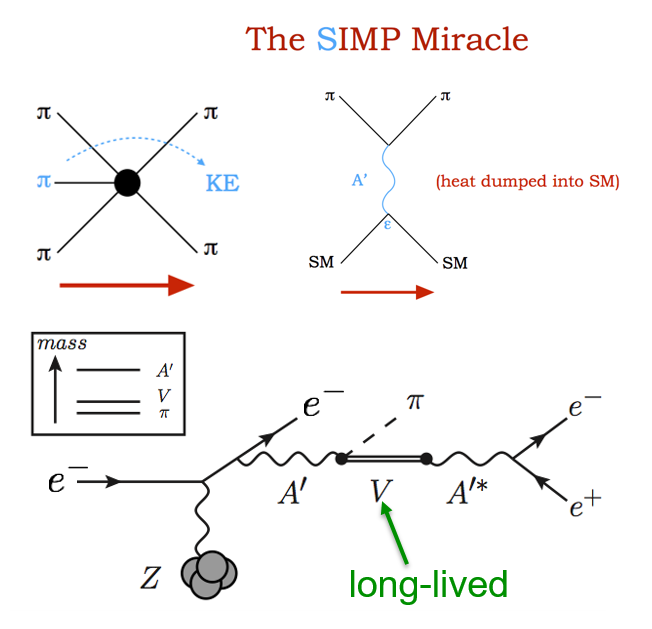
\includegraphics[width=0.85\textwidth]{figs/upgrades/simpmiracle.png}
    \caption{A mechanism in the early universe in which dark pions undergo a $3 \rightarrow 2$ annihilation mechanism followed by heat being dumped into SM sector to produce the cold dark matter observed today. This mechanism can be tuned to achieve the correct dark pion relic abundance of dark matter and is known as the ``SIMP Miracle.'' This motivates a dark matter mass in the range $\sim 10 - 100$ MeV. HPS can probe the production the mechanism $e^-Z \rightarrow e^-Z\aprime$ and then $\aprime \rightarrow \pi_D V_D$ and then $V_D \rightarrow \epem$ where the $V_D$ is long-lived.}
    \label{fig:simpmiracle}
\end{figure}

These parameters are not completely free and are bound by constraints, motivations, and dependencies that arise from quantum field theory and cosmology. Additional constraints come from the limitations of HPS and are as follows:

\begin{enumerate}
  \item The gauge coupling $\alpha_D$ is only constrained by perturbativity to be less than 1. Naturalness arguments will put $\alpha_D \sim 10^{-2}$; however, this constraint can be easily be relaxed in order to probe the full parameter space.
  \item The requirement from SIMP cosmology sets a lower bound on the kinetic mixing parameter $\epsilon > 10^{-6.3}(m_{\aprime}/10^{-2} \ \mathrm{GeV})^{1/2}$ for $\alpha_D = 10^{-2}$ and the mass ratio used below.  Larger couplings ($\epsilon \sim 10^{-5}-10^{-3}$) are allowed if a kinetic mixing loop arises from massive particles charged under both the dark $U \prime (1)$ and the SM hypercharge. For even larger couplings ($\epsilon > 10^{-2}$), the model approaches the standard scalar thermal dark matter scenario as $\pi_D$ annihilations through the $\aprime$ significantly impact the dark matter relic abundance.
  \item Pertubativity requires the ratio $m_{\pi_D}/f_{\pi_D} < 4 \pi$. An additional constraint from the dark matter relic abundance from $\pi_D$ together with fixed $V_D$ and $\pi_D$ masses also fixes the ratio $m_{\pi_D}/f_{\pi_D}$ which is shown in Fig. \ref{fig:simpbr}.
  \item For SIMP cosmology to work, certain annihilations such as $\pi_D \pi_D \rightarrow A^{\prime*} \rightarrow \bar{f}f$ and $\pi_D \pi_D \rightarrow \aprime \pi_D$ should be suppressed which is achieved by requiring $\epsilon < 10^{-2}$ and $m_{\aprime}>2m_{\pi_D}$, respectively.
  \item HPS can only search for visible decays into $\epem$ pairs which this requires $V_D > 2m_e$. The $\aprime$ decay channel requires $m_{\aprime}>m_{\pi_D} + m_{V_D}$.
  \item Effective field theory provides a rough prediction relating the ratio of the dark vector mass to the dark pion mass.
  \begin{equation}
    \frac{m_{V_D}}{m_{\pi_D}} \sim \frac{4 \pi}{\sqrt{N_c}(m_{\pi_D}/f_{\pi_D})}
    \label{eqn:mvdmpid}
  \end{equation}
  where $N_C$ is the number of colors in the dark QCD. As in the SM, $N_C=3$ and vector mesons are heavier than pions. Enforcing this relationship further reduces the number of independent parameters and is shown to be generally independent of $m_{\pi_D}/f_{\pi_D}$ in Fig. \ref{fig:simpbr}.
\end{enumerate}

In order to ensure visible decays, which is required by HPS and not by the theory, the mass hierarchy is required to be $m_{\aprime}>m_{V_D}+m_{\pi_D}$ and $m_{V_D}>2m_e$. Assuming the same dark bremsstralung production mechanism of $\aprime$s as described in Sec. \ref{sec:signatures}. Once an $\aprime$ is electro-produced, it can decay into some combination of dark vectors and dark pions \cite{Hochberg2016}. The decay width of an $\aprime$ decaying into two dark pions $\pi_D$ is:

\begin{equation}
    \Gamma (\aprime \rightarrow \pi_D \pi_D)  = \frac{2 \alpha_{D}}{3} m_{\aprime} \left( 1-\frac{4 m^2_{\pi_D}}{m_{\aprime}^2}\right)^{3/2} \left( \frac{m_{V_D}^2}{m_{\aprime}^2-m^2_{V_D}}\right)^2
    \label{eqn:pipi}
\end{equation}

This mechanism leaves the recoil electron as the only visible particle in the final state. Thus, this $\aprime$ decay cannot be probed with HPS. The decay width of an $\aprime$ into a dark pion and a dark vector $V_D$ is:

\begin{equation}
    \Gamma (\aprime \rightarrow V_D \pi_D)  = \frac{\alpha_D T_V}{192 \pi^4} \left( \frac{m_{\aprime}}{m_{\pi_D}} \right)^2 \left( \frac{m_{V_D}}{m_{\pi_D}} \right)^2 \left( \frac{m_{\pi_D}}{f_{\pi_D}} \right)^4 m_{\aprime} \beta (x,y)^{3/2}
    \label{eqn:Vpi}
\end{equation}

where $x=m_{\pi_D}/m_{\aprime}$, $y=m_{V_D}/m_{\aprime}$, and  $\beta(x,y)=(1+y^2-x^2-2y)(1+y^2-x^2+2y)$. The variable $T_V$ is a function of the dark meson flavor.

\begin{equation}
    T_V = \left\{
    \begin{array}{ll}
    3/4, & \mbox{if $\rho$} \\
    3/2, & \mbox{if $\phi$} \\
    18, & \mbox{otherwise}.
    \end{array}
    \label{eqn:Tv}
\end{equation}

The dark pion is invisible and is not reconstructed for HPS. Thus, it will appear as missing energy, and the $\epem$ momentum sum will not peak at the beam energy as with $\aprime$s. In fact, the search for SIMPs is performed in a mutually exclusive parameter space in momentum sum as shown in Fig. \ref{fig:simplivetime}. Finally, for $m_{\aprime}>2m_{V_D}$ the decay into two dark vectors is allowed with a decay width of:

\begin{equation}
    \Gamma (\aprime \rightarrow V_D V_D)  = \frac{\alpha_D}{6} f(r) m_{\aprime}
    \label{eqn:VV}
\end{equation}

where $r=m_{V_D}/m_{\aprime}$ and

\begin{equation}
    f(r) = \left( \frac{1+16r^2-68r^4-48r^6}{(1-r^2)^2} \right) \sqrt{1-4r^2}
    \label{eqn:fr}
\end{equation}

As will be described, each $V_D$ will decay into $\epem$ pairs for $2m_e<m_{V_D}<2m_{\mu}$ thus this last decay will have a four lepton final state. The acceptance of HPS to a four lepton final state is small, but has not been carefully evaluated. To increase the difficulty for searches at HPS, such a mechanism would include two secondary vertices which would be challenging to resolve if only a fraction of the particles are within HPS acceptance. For these reasons, this mechanism is not explored and the focus is on the $\epem \pi_D$ final state.

Finally, the same decay width of $\aprime \rightarrow \epem$ for the canonical $\aprime$ model is used but is small compared to the other decay widths. Once again assuming $2m_e<m_{V_D}<2m_{\mu}$, the decay width of $V_D$ is:

\begin{equation}
    \Gamma(V_D \rightarrow \epem) = \frac{16 \pi \alpha_D \alpha \epsilon^2 f^2_{\pi_D}}{3m^2_{V_D}} \left( \frac{m^2_{V_D}}{m^2_{\aprime}-m^2_{V_D}} \right)^2 \sqrt{1-\frac{4m_e^2}{m^2_{V_D}}} \left( 1+ \frac{2m_e^2}{m^2_{V_D}}\right) m_{V_D} \times x
    \label{eqn:vdecay}
\end{equation}

where $x = 2$ for a dark $\rho$ and $x= 1$ for a dark $\phi$ (the only two dark mesons of interest). Decays into SM hadrons and muons are not explored in this work because the mass hierarchy kinematically forbids such decays.

From the decay widths, the livetimes can be trivially computed and are shown in Fig. \ref{fig:simplivetime}. Note that the additional parameters in the SIMP model decouple the livetime and production cross-section such that it is possible to have a high rate of long-lived particles. This is opposed to the canonical $\aprime$ model which have coupled livetimes and cross-sections and is ideal for HPS.

For this study, to further reduce the number of parameters, a fixed ratio of the masses of the three new particles is fixed. The ratio of $m_{\aprime}:m_{V_D}:m_{\pi_D}$ is chosen to be $3.0:1.8:1.0$ which respects the constraints required for a visible signal at HPS and also kinematically forbids a $\aprime \rightarrow V_D V_D$ which complicates the search as previously described. This ratio also respects the relation described in Eq. \ref{eqn:mvdmpid}. In addition, the other observables are the livetimes and cross-sections which can be trivially reweighted after MC reconstruction. Thus, with the fixed mass ratio and reweighting scheme, the model can effectively reduced to two parameters - $m_{\aprime}$ and livetime.

\begin{figure}
    \centering
    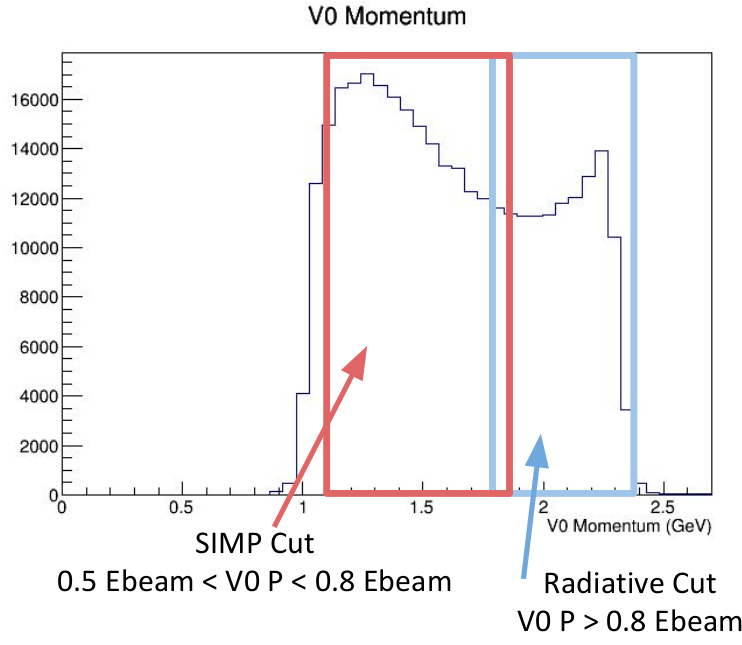
\includegraphics[width=0.45\textwidth]{figs/upgrades/simp_p.png}
    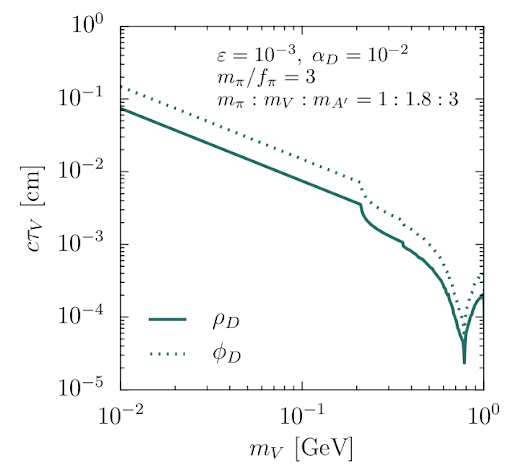
\includegraphics[width=0.45\textwidth]{figs/upgrades/simp_lt.png}
    \caption{Left: The reconstructed V0 momentum that shows roughly the different parameter space for canonical $\aprime$s and SIMPs. The lower momentum sum of the SIMP parameter space is due to missing energy from the dark pion. Right: The livetime ($c\tau$) of two dark mesons ($\rho_D$ and $\phi_D$) for a given set of parameters. The livetime $c\tau \sim 0.1 - 10$ mm is within HPS range.}
    \label{fig:simplivetime}
\end{figure}

\begin{figure}
    \centering
    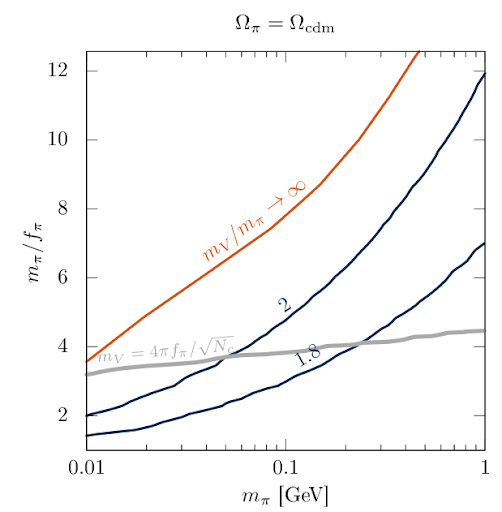
\includegraphics[width=0.45\textwidth]{figs/upgrades/mpifpi.png}
    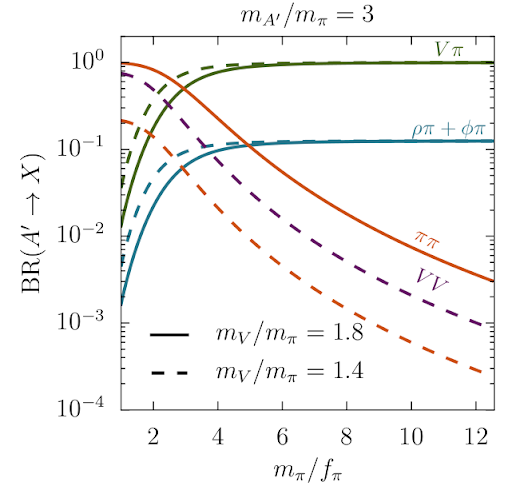
\includegraphics[width=0.45\textwidth]{figs/upgrades/simp_br.png}
    \caption{Contours in the $m_{\pi_D}-(m_{\pi_D}/f_{\pi_D})$ space for different choices of $m_{V_D}/m_{\pi_D}$ assuming $\pi_D$ makes up all the dark matter. Right: The branching ratio as a function of $m_{\pi_D}/f_{\pi_D}$. For HPS, the branching ratio in the parameter space of interest for the sum of $\rho_D$ and $\phi_D$ is about $\sim$10\%.}
    \label{fig:simpbr}
\end{figure}

%\subsection{SIMP Projections}\label{sec:simpreach}

Using these constant mass ratios, the projections for $\alpha_D=0.01$  and $m_{\pi_D}/f_{\pi_D}=3, \ 4\pi$ are shown in Fig. \ref{fig:simpreach}. Because of the livetime dependence on these parameters and their wide range of possible values, the expected number of displaced events varies by several orders of magnitude in the parameter space of interest. In general, the number of expected signal events increases with increasing $m_{\pi_D}/f_{\pi_D}$ and decreasing $\alpha_D$. These projections show that HPS potentially has sensitivity to new territory for a wide range of motivated parameter space of the SIMP model with the data from the 2016 Engineering Run.

\begin{figure}
    \centering
    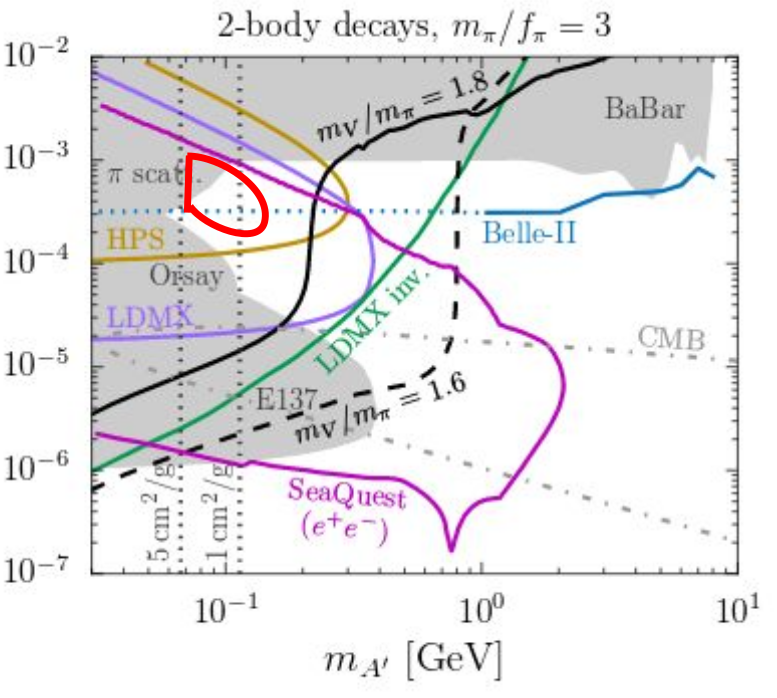
\includegraphics[width=0.45\textwidth]{figs/upgrades/simpreach1.png}
    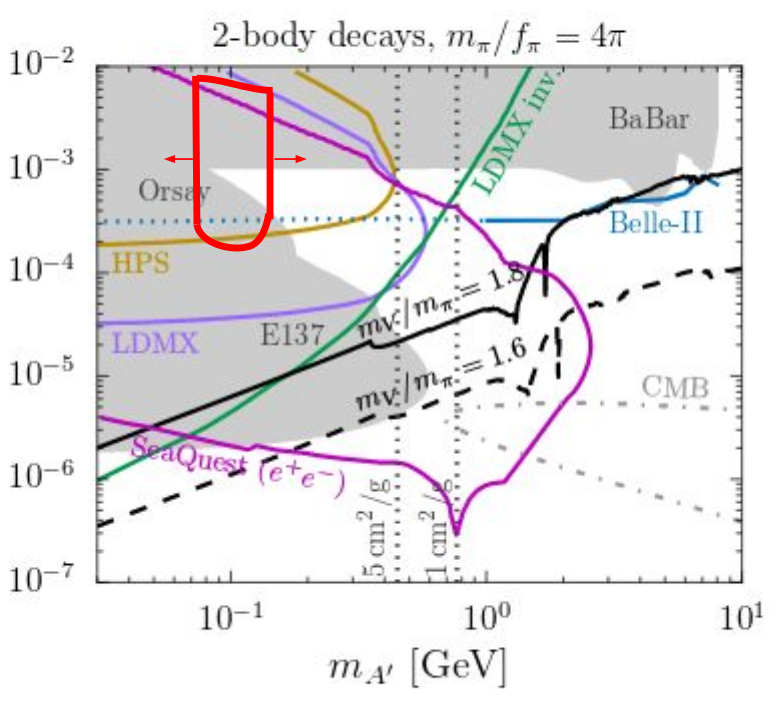
\includegraphics[width=0.45\textwidth]{figs/upgrades/simpreach2.png}
    \caption{The SIMP reach estimate from the full 2016 Engineering Run dataset shown in $\epsilon^2$ - $m_{\aprime}$ space for $\alpha_{dark}=0.01$ and for Left: $m_{\pi_D}/f_{\pi_D}=3$ and Right: $m_{\pi_D}/f_{\pi_D}=4\pi$. The ratio of the masses is kept constant at $m_{\aprime}:m_{\rho}:m_{\pi_D}=3.0:1.8:1.0$ for simplicity. The contours in red are drawn at 2.3 expected events and the dataset is projected to set new limits in previously unprobed territory. The contours in yellow are from theory calculations.}
    \label{fig:simpreach}
\end{figure}


